\documentclass[12pt]{article}

% Set up data, if you need to add a package, go here
%Adapted from Adapted from UWA Engineering Final Year Project.


\usepackage[utf8]{inputenc}
\usepackage[x11names,dvipsnames,svgnames,table]{xcolor}

% general incantations
\usepackage[export]{adjustbox}
\usepackage{afterpage}

\usepackage{graphicx}
\usepackage{placeins}
\usepackage{pdfpages}
\usepackage{algorithm2e}
\usepackage{array}
\usepackage{booktabs}
\usepackage[most]{tcolorbox}
\usepackage{calligra}
\usepackage{caption}
\usepackage{datetime}
\usepackage{dblfnote}
\usepackage{dirtytalk}
\usepackage{dsfont}
\usepackage{etex}
\usepackage{fancyhdr}
\usepackage{fix-cm}
\usepackage[T1]{fontenc}
\usepackage{textcomp,gensymb} %for \degree C symbol
\usepackage{graphicx}
\usepackage{lipsum}
\usepackage{listings}
\usepackage{transparent}
\usepackage[everyline=true,framemethod=tikz]{mdframed}
\usepackage{mparhack}
\usepackage{multicol}
\usepackage{multirow}
\usepackage{parskip}
\usepackage{lscape}
\usepackage{pdflscape}
\usepackage{pdfpages}
\usepackage{placeins}
\usepackage[document]{ragged2e}
\usepackage{rotating}
\usepackage{setspace}
\usepackage{subcaption}
\usepackage{threeparttable}
\usepackage[normalem]{ulem}
\usepackage{verbatim}
\usepackage{soul} %highlighting, strike through etc.
%\usepackage{float}

%Automated appendices
\usepackage[titletoc,title,header]{appendix} %advanced functionality

%language settings
\usepackage[utf8]{inputenc}
\usepackage[australian]{babel}
\usepackage{csquotes}

%page setup
%this where we adjust the binding offset, if relevant
\usepackage[a4paper]{geometry}
\usepackage{lastpage} % for page 1 of n footers

%cross referencing
\usepackage[hidelinks]{hyperref}
\usepackage{cleveref}

%maths stuff
\usepackage{amsmath}
\usepackage{mathtools}

\setcounter{secnumdepth}{5}

%lists
\usepackage{enumitem}

%working collaboratively
\usepackage[backgroundcolor=yellow]{todonotes}

% bibliography file using harvard
\usepackage[style=authoryear-ibid,backend=biber]{biblatex}
\bibliography{bibliography.bib} % with extension

%glossary for acronyms
\usepackage[acronym,nonumberlist,toc,section=subsection,numberedsection=nolabel]{glossaries}
\makeglossaries

%line spacing
\linespread{1.25}

\begin{document}


\thispagestyle{empty}
\setlength\headheight{0pt} 
\begin{center}

\begin{center}

\includegraphics[width=0.65\linewidth]{resources/TUD_Logo.png}
\end{center}	

        \vspace{0.25cm}
        {\scshape\LARGE TU Dublin, Tallaght Campus \par}
        \vspace{0.25cm}
        {\scshape\Large Research Project, M.Sc. in DevOps\par}
        \vspace{0.5cm}

        {\Large\bfseries Evaluating the Next Generation Sidecar-less Kubernetes Service Mesh: Ambient Mesh\par}
        
        \vspace{0.5cm}
        {\Large\itshape Anupam Saha\par}
        Department of Computing
        \vspace{0.25cm}

\vspace{1cm}
Supervised by\par
Dr. John Burns \\
Department of Computing\par
\vspace{1.5cm}
\large
\today

\end{center}

\clearpage
\restoregeometry
\justify

\section*{Declaration}
I hereby certify that the material, which I now submit for assessment on the programmes of study leading to the award of Master of Science, is entirely my own work and has not been taken from the work of others except to the extent that such work has been cited and acknowledged within the text of my own work. No portion of the work contained in this thesis has been submitted in support of an application for another degree or qualification to this or any other institution.

\vspace{2cm}
\begin{flushright}
-----------------------------------\\
Anupam Saha\\
\today
\end{flushright}
\pagebreak

\section*{Acknowledgements}
First and foremost, I want to sincerely thank Technical University of Dublin and the ICT Skillnet teams for providing this amazing chance to be a part of the Master's program. I also like to express my gratitude to Dr. John Burns, my supervisor, for his insightful criticism and suggestions on this dissertation. In closing, I would like to express my gratitude to my family and friends for their unwavering support over this extremely demanding academic year.
\pagebreak

%List of figures and tables, automatic from thesis.
\listoffigures
\pagebreak


\listoftables
\pagebreak



\newacronym{boa}{BOA}{Bank of Anthos}
\newacronym{gcp}{GCP}{Google Cloud Platform}
\newacronym{gke}{GKE}{Google Kubernetes Engine}
\newacronym{vpc}{VPC}{Virtual private network}
\newacronym{iac}{IaC}{Infrastructure as code}
\newacronym{rbac}{RBAC}{Role based access control}

\newglossaryentry{wireshark}{name=Wireshark,description={A open source network packet filtering tool}}


\printglossary[type=\acronymtype]
\pagebreak


\tableofcontents
\pagebreak


\section*{Abstract}
Over the last few years service mesh has become an essential part of the cloud native stack. A service mesh is a dedicated infrastructure layer in Kubernetes cluster to make service-to-service communication safer, faster, and reliable. There are number of established service mesh products used today including Istio, a project developed by Google, IBM and Lyft, the company behind envoy proxy. Istio provides a two tier architecture consisting a control and data plane. The data plane is implemented by injecting envoy proxies as a sidecar container to microservice pods to deliver service mesh capabilities. This sidecar containers require additional compute resources to run and impacts the Istio system efficiency in many situations. Hence, a new data plane architecture in Istio was born as Ambient mesh. The new data plane provides service mesh capabilities without sidecar injection and claims to achieve greater efficiencies. With the release of ambient mesh alpha version as part of Istio, the potential of this sidecar-less architecture is explored in gray literature, but no academic paper is produced. The aim of this paper is to evaluate the resource utilization and operational experience improvement of ambient mesh by comparing Istio sidecar and ambient modes on Google Cloud Platform. Multiple test scenarios covering a variety of deployment models shows a significant improvements in resource consumption of Istio system in ambient mode. Operational experience is also improved in Istio ambient mode by having a declarative method for installation and upgrade which does not require a microservice pod restart. Additionally the segregated data plane layers of ambient mesh helps in gradual service mesh adoption. Finally the research concludes that a shift towards this new architecture is significant provided a stable version of ambient mesh is released which will open further research avenues.
\pagebreak


\section{Introduction}
\subsection{Service Mesh and Istio}
When the industry moved from monolith to microservice architecture a decade ago, additional challenges has been introduced. Some of the most prominent were service discovery, secure communication between microservices, policy enforcement and monitoring multi fold micro-services for a single application. All these non-functional requirements easily became the overhead for many development teams and service mesh concept was introduced as path to mitigation. Istio is one of the most popular implementation of such concept which is heavily used in current cloud enabled businesses.

At the core of Istio, it uses sidecar proxies which encapsulates all the methods to implement the non-functional requirement without microservice code being impacted (\cite{techcrunch2022}). The sidecar sits as a separate container in microservice host or Kubernetes pods to intercept all the traffic requests and establish communication, network policy and security practices that the business expects from any service. In this architecture, additional containers are deployed alongside with service containers hence it increases the latency and resource utilization of the application. Despite of the minimal extra resource usage the functionality and reliability these containers provide are inevitable.

\subsection{Motivation}
Performance optimization remains an engineering tasks for any software team and service mesh is no different. There has been several literature published on comparing Istio and other service meshes from performance and security perspective but there is no paper which describes a different architecture for service mesh altogether. Most of the service mesh available in the market either use Envoy or in-house developed sidecar proxies which incorporates the success factor for the product but a very few effort has been made to invent a solution from ground up. This paper explores one of such way to change the current service mesh is architect and configured to run on Kubernetes environment.

\subsection{Research Questions}
The following questions were formulated for the purpose of this research:
\begin{itemize}
\item Does the ambient mesh consumes less compute resources than Istio's sidecar mode?
\item Does the sidecar less architecture reduces operational complexities?
\end{itemize}

\subsection{Objectives}
The objective of this research is to establish the followings:
\begin{itemize}
\item Comparison of CPU and memory utilization between Istio standard and ambient mode
\item Verify whether the ambient mode introduces any extra latency between microservice calls
\item Compare the Istio system roll out and upgrade complexity between Istio standard and ambient mode
\end{itemize}
\pagebreak


\section{Literature Review}

\subsection{Background}
Practitioners quite often run into an exaggeration of past issues while trying to leverage recent technologies in a rapid pace. In cloud native world the network is unreliable, thus while developing bigger and more dispersed systems, the network needs to be taken into account from the outset of application design (\cite{posta2022Design}). Implementing network resilience like retries, timeouts, circuit breakers, observability and security became challenging for application developer hence a decentralized application networking infrastructure was born as service mesh. Istio is one such open source implementation which has been used for a while now and battle tested by many corporations with their business deliveries. Istio specifies an architecture consisting of a control plane for proxy management and a data plane for network traffic and security management on behalf of an application using application layer proxies (\cite{posta2022Layers}). These application-layer proxies sits as a sidecar within the Kubernetes environment and attached to each service workloads making it a tightly coupled relation with the service deployments. Istio's sidecar proxy injection provides significant advantages over microservice code refactoring for non functional requirements, but do not offer a perfect separation between applications and the Istio data plane (\cite{istioHoward2022}). The Istio community practitioners and contributing companies explored the options of having a less invasive and better ergonomic approaches in service mesh  from last couple of years and Ambient mesh was born. It is now possible to get rid of sidecar architecture in Istio by introducing a shared agent model running per host wise. This gives the operator a lot of cost benefit, flexibility and also provide interoperability with previous generations of service meshes with sidecars. Essentially ambient mesh brings a lot of new excitements in the service mesh space without compromising any purposes that it was invented for.

\subsection{Service Mesh Origins}
During the early days of the Internet, applications used to ship their own TCP/IP stack. This implies that all networking layer code either used to be packaged with the applications or the language specific libraries used to be linked with the application binaries. With the next generation of application development people started shifting towards a shared library model which is still the case with many desktop or embedded applications. Then the creation of the three-tiered application architectural paradigm, which served as the basis for the vast majority of web applications followed by the service-oriented architecture changed the techies to think the way they handled things previously. With this new decoupled service-oriented architecture, additional requirements related to visibility, connection, and security have emerged. Resiliency became more and more important including application components communication over non trusted networks beyond cloud and premises boundaries, and security advancement to a point where sender and recipient can authenticate each other's identities.

\begin{figure}[ht!]
    \centering
    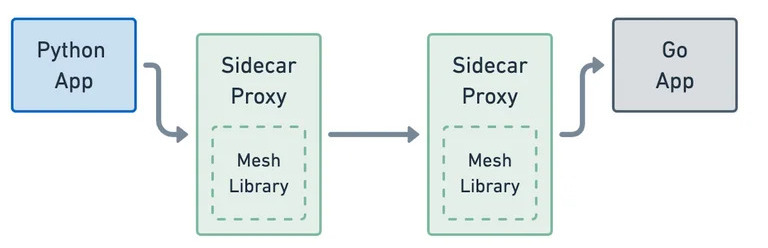
\includegraphics[width=0.7\linewidth]{resources/sidecar-design.jpg}
    \caption{Sidecar proxy design (\cite{isovalentGraf2021})}
    \label{lr:sidecarDesign}
\end{figure}

Implementing all these functionalities out of the application or shared libraries was a big task and making them available as part of the infrastructure for use by all applications was another big challenge. As a solution, sidecar model was introduced which eliminates the need to modify each application separately and supported the polyglot nature of microservice development to best suite the business needs or expertise. The term 'sidecar' was adopted as it attached to the microservices much like a sidecar attached to a motorcycle. This sidecars are now placed with each Kubernetes workload to anticipate network or security movements inside a cluster to form a service mesh delivering speed to the development teams to focus on business logic. Overall, service mesh is a way to connect multiple services to one consistent network and observability layer (\cite{posedioNeumer2021}).

\subsection{Moving from Shared Library Model to Kernel Model - Check}
\label{lr:ebpf}
Historically, the operating system has always been an ideal place to implement observability, security, and networking functionality (\cite{ebpfIODocs}). As operating system implements the central controller unit called kernel, it holds the unique capacity of monitoring and managing the entire system. Over the period of time innovation at kernel level has been lower as its tend to be more complex than functionality outside of it, but with eBPF, that has changed in last few years. What JavaScript did to the browser to change the way today's web application works, eBPF is doing the same at Linux Kernel space. eBPF is a revolutionary technology that runs sand-boxed programs in kernel without modifying the kernel source code or injecting an external kernel module to extend its functionality. Essentially, its a run time in kernel including a JIT compiler to compile byte codes into machine code for execution, making it very optimized and similar level of performance as  native kernel code. eBPF adds the dynamic ability to program kernel by removing back and forth calls between kernel and user space. eBPF works at kernel and user space level by a event driven hook pattern. These events include the entry or exit from any routine in kernel or user space, trace points, and most importantly the arrival of network packets which is crucial for any service mesh (\cite{thenewstackRice2021}). This makes eBPF extremely useful at host level networking observability, security and traffic management.

\begin{figure}[ht!]
    \centering
    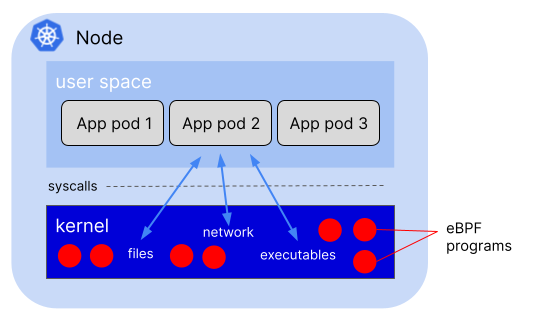
\includegraphics[width=0.7\linewidth]{resources/ebpf-service-mesh.png}
    \caption{eBPF implementation of service mesh (\cite{thenewstackRice2021})}
    \label{lr:ebpfDesign}
 \end{figure}

 As there is only one kernel per Kubernetes nodes, this eBPF technology has become prominent for the service mesh development as this allows to have only one dynamic program for the kernel to serve the service mesh functionalities. This eBPF application program acts as a proxy, but in this case instead of attaching to each pods in Kubernetes cluster, it is attached to the Kubernetes nodes kernel. When attaching proxy to the kernel, a one to one mapping is formed between kernel and proxy eliminating the need of injecting sidecar proxies per pod wise. The evolution from shared library to sidecar and now the kernel model for non-functional requirements in applications development have really gone through a massive change and at each stage the significance was clearly seen by the practitioners.

\subsection{Ambient Mesh Architecture}
With Istio 1.18.0 release in June 2023, the first alpha version of Ambient mesh is launched. This new release gives an option to run Istio installation with ambient parameter to forgo sidecar proxies in favor of a mesh data plane integrated into Kubernetes infrastructure (\cite{istioHoward2022}). To understand Ambient mesh architecture a quick look into Istio sidecar or standard architecture is required. Istio standard has a data plane and a control plane. The data plane is the sidecar proxy which is injected to each Kubernetes pods to monitor, handle and response to events and provide necessary details to and from the service to the mesh network. Control plane remains the controller unit for these data planes and generally its centrally located in the cluster. Ambient mesh divides the data plane into two segments, secure overlay layer or L4 processing layer and L7 processing layer. This layering gives the flexibility to the operator to use the basic potential of a service mesh by deploying L4 processing layer only, reducing the overhead to the entire Kubernetes cluster. The layered approach also helps in migration from no mesh system to secure overlay and to full L7 processing. Next two paragraphs will explore these layers along with the Ambient mesh components which forms the sidecar less architecture.

\subsubsection{L4 Secure Overlay Layer}
Layer 4 of the OSI model represents the transport layer which provides a transparent view of data transfer between end users. Traditionally service mesh incorporates both L4 transport layer and L7 application layer in a single sidecar entity, but in Ambient mesh this is separated and a new zero trust proxy or Ztunnel is introduced. This component is written from ground up using one of the most efficient programming language Rust which naively supports network optimizations and packet filtering. Ztunnel concentrates on a limited number of capabilities, such as mTLS, authentication, L4 authorization and telemetry for Kubernetes workloads without interrupting or processing application level HTTP headers (\cite{istioSun2023}). Ztunnel is deployed as a daemon set on every Kubernetes nodes to process the basic service mesh capabilities. It also forwards the request to the intended app after gathering L4 metrics such as the quantity of request or response bytes. When the target application is running on a different node it ensures that the data is sent to the respective Ztunnel over a secure mTLS connection. The following diagram illustrates how Ztunnel intercepts communication for every pod that is deployed on the same node.

\begin{figure}[ht!]
    \centering
    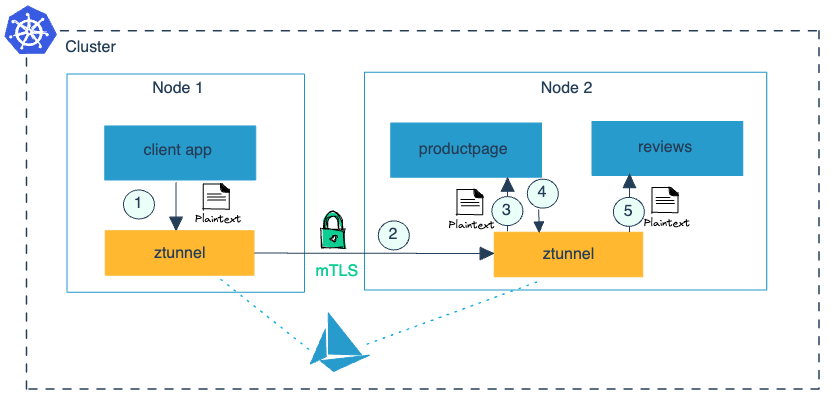
\includegraphics[width=0.7\linewidth]{resources/ambient-routing-l4.png}
    \caption{In cluster routing with Ztunnel in Ambient mesh}
    \label{lr:ztunnelDesign}
 \end{figure}

 \ref{lr:ztunnelDesign} depicts how a client application accept requests from end user to serve a product page along with its reviews. The application runs on a Kubernetes cluster with 2 nodes where the UI, product and review microservice pods are spread across multiple nodes. Each node has its own Ztunnel which internally communicates over mTLS to provide a response back to the end user.

 \subsubsection{L7 Processing Layer}
 Layer 7 works at the highest level of OSI model where application details are available, hence a detailed HTTP level filtering can be done. L7 processing is intensive as it intends to provide connectivity, shape the traffic, apply policies and provide mTLS for microservices running across nodes. This intensive layer analyzes a lot of data and processes a massive scale of network traffic utilizing more CPU and memory resources. To reduce this burden, Ambient mesh introduces a shared component called Waypoint proxy which works at per namespace or per Kubernetes service account level. Waypoint proxies are deployed as a pod and can be placed in any Kubernetes nodes irrespective of where the microservice pods are hosted. The Waypoint proxy forwards the request to the Ztunnel running on the same or different node as the destination microservice, but not before enforcing the L7 rules and gathering L7 metrics (\cite{glooDocs}). By default, mTLS is used to secure traffic between Ztunnel and the Waypoint proxy.

 \begin{figure}[ht!]
    \centering
    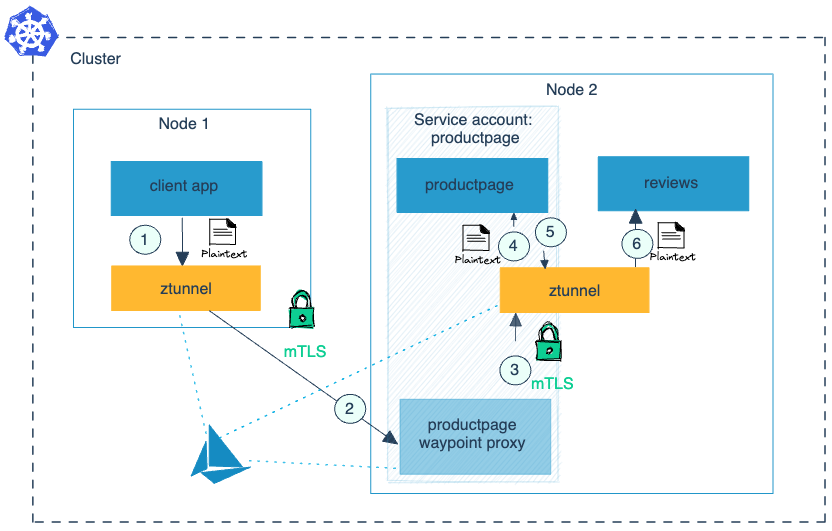
\includegraphics[width=0.7\linewidth]{resources/ambient-routing-l7.png}
    \caption{L7 routing in Ambient mesh}
    \label{lr:waypointDesign}
 \end{figure}

 As shown in the above diagram, the Waypoint proxy is deployed in the product page service account. The request from client application first reaches to the Ztunnel of the client app and then routed to the Waypoint proxy. This is possible as L7 traffic policies are applied to the product page. On receiving the request, Waypoint proxy performs the L7 processing such as collecting metrics and forwards it to the Ztunnel of the corresponding node where the product page microservice pod is running.

 \subsection{Value Proposition of Ambient Mesh}
 A few grey literature describes, using sidecar less model one can reduce the number of proxy instances significantly. One of the empirical study (\cite{thenewstackRice2021}) mentions about using a service mesh built on top of eBPF technology can cut down the proxy counts from 100 to just 3 in a complex Kubernetes cluster used in production. In some other articles, the problem of sidecar proxies are discussed from a real life scenario. \cite{mediumSinghal2021} mentions how they faced an massive increase in memory usage per proxy from 60 - 70MiB to 700MiB - 1.2GiB when they shifted from a small Kubernetes cluster to a larger one. The root cause was identified in the same article and the solution was to restrict the proxy to the required namespaces so that it does not ingest network traffic data for all the services running in the cluster. But even with this limited proxy configuration, per node memory utilization could reach up to a significant number when the service replica increases due to auto scaling. Kernel mode service mesh not only reduces this memory footprint, but it can also reduce the complexity of having less YAML, application pod restart when rolling out the service mesh in a live cluster. Though the focal point of the kernel mode service meshes like Ambient mesh remains at the performance side but the reduced operational complexities can not be ignored. One of the most significant benefits of switching to Ambient mesh is two layers of network traffic filtering. Ambient mesh allows incremental adoption by applying secure overlay processing by default and high level HTTP based L7 processing on demand. This two layer architecture enables organizations to pay for what is needed and scale the service mesh data plane independently from the Kubernetes workload reducing the infrastructure cost (\cite{infoqSunCampbell2023}).

 \subsection{Summary}
 Ambient mesh offers advantages over sidecar based deployment model due to its noninvasive and leaner design. Adoption of the ambient mesh directly reduces infrastructure costs and improves performance because it involves fewer components - Ztunnel proxies per node and the optional Waypoint proxy. The design also allows for separating L4 and L7 processing, giving the operator a granularity on control and choice. Though the introduction of Ambient mesh does not mean the end of sidecar model in service mesh, there is a lot of potential which Ambient mesh brings today. There are use cases when service meshes with sidecar may remain useful such as in regulatory environments as keeping proxies in the same pod guarantees to be coupled with microservice at the same geographic location which is easy to justify during an audit. Despite of few exceptional cases, ambient mesh will remain as one of the most exciting technology in service mesh field which leverages the Linux kernel eBPF technology. As there is no academic research paper available at present, an immense opportunity is opened to explore Ambient mesh, what it offers and how it is different from standard sidecar mode of Istio.
\pagebreak


\section{Method}

\subsection{Cloud Infrastructure}
Public cloud being the most preferred choice for enterprise grade application deployments where the microservice communication and security is handed over to Istio, this research is conducted on \acrlong{gcp}. \acrshort{gcp} remains the choice as public cloud provider for this research project mainly because of the author's familiarity with the platform. As Istio works at Kubernetes environment level, all the methods used in this research are conducted on \acrlong{gke} - the fully managed Kubernetes service offered by \acrshort{gcp}.

\subsubsection{High Level Strategy}
To maintain a consistent and steady approach for each deployment and testing stages, \acrfull{iac} is used with Terraform. A rapid cloud infrastructure provisioning and de-provisioning model is followed to keep the cloud cost minimal. All the Terraform IaC, Shell scripts and Kubernetes configurations files used in this research are available at \ref{appendix:researchRepo}. At a high level first the Kubernetes cluster is provisioned and verified by kubectl on local system. Next the observability stack is installed on the cluster followed by the service mesh itself is installed and verified. After all the platform level stuffs are installed, configured and verified, a demo web application \acrfull{boa} is deployed using Kubernetes manifest files including the front end microservice attachment to the Istio ingress controller. This enables the application to be accessed from outside of the cluster. At the end of each testing sessions, everything is teared down completely using \acrshort{iac} to save cloud cost.

\subsubsection{Terraform Provisioning}
Google offers several Terraform APIs to customize the cluster resource provisioning which gives a greater control and flexible management of \acrshort{gke} cluster. As a prerequisite of Terraform provisioninig a GCP project and service account is created manually from \acrshort{gcp} console along with enabling all required APIs using gcloud command line tool on local system. \acrfull{iac} used in this research leverages several Terraform modules to provision the \acrshort{gke} cluster along with necessary cloud components like \acrshort{vpc} network, subnet and node pool. Terraform script defines the following configurations for the cluster creation.
\begin{itemize}
  \item GCP europe-west1-b zonal cluster
  \item e2-standard-2 machine type with 2 vCPU and 8GiB RAM
  \item Latest stable release of Kubernetes v1.27.3
  \item Node scaling from 1 to 10 with an initial count of 2
\end{itemize}

Essentially, a zonal cluster is created in europe-west1 physically located at Belgium (\cite{gcpDocRegion}) to keep the cloud cost to minimal. The default node pool comes with a cluster is not used here to define some custom parameters like manual IP ranges for Kubernetes services and pods, lower disk size. Selecting the machine type as e2-standard-2 gives \acrshort{boa} an ample amount of resources along with Istio components. Kubernetes version is set to v1.27.3 which is one of the most recent and stable release of Kubernetes (\cite{kubeDocRelease}) at the time of writing this paper.


\subsubsection{Demo Application}
\acrshort{boa}, a microservice based demo application from \acrshort{gcp} open source repository \cite{githubBOA} is used for this research project. This application is developed by \acrshort{gcp} team to demonstrate their products and proven to be a perfect fit for evaluating Ambient mesh as it comes with predefined Kubernetes deployment manifest files. With minimal changes to these manifest files, microservice deployment remains fairly straight forward job for the research. This enables focusing more on the Istio rather investing more time on application source code build and deployment. \acrshort{boa} simulates a virtual online banking system with facilities of account opening, deposit, withdraw and balance enquiry. This application consists of a total nine microservices out of which, eight microservices are used without any modifications for this research. The application follows a typical microservice based architecture which is defined in Figure \ref{method:boaDesign}.

\begin{figure}[ht!]
  \centering
  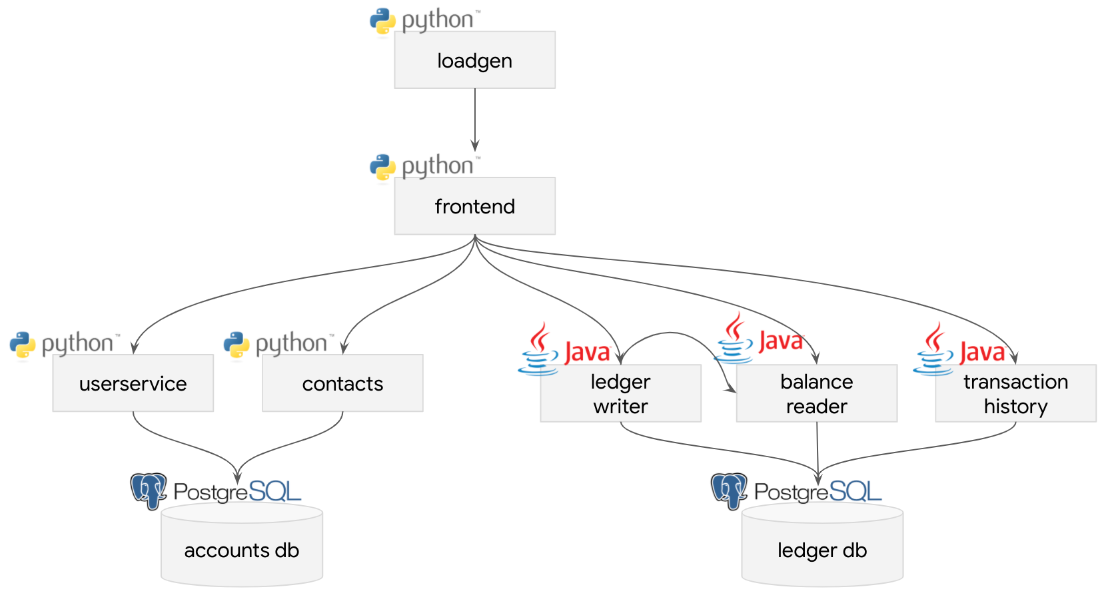
\includegraphics[width=1.0\linewidth]{resources/boa-architecture.png}
  \caption{Bank of Anthos application architecture}
  \label{method:boaDesign}
\end{figure}

The load generator script comes with the project is modified to suite the purpose of this research and run from local system to reduce the burden on the cluster.


\subsection{Observability Mechanism}
\label{observabilityStack}
Monitoring in dynamic service-oriented architectures is a crucial point of success and observability takes it all to a complete new level by exploring the internal state of the microservices. This paper explores the resource utilization of ambient mesh in different conditions and compares them with Istio's sidecar models utilization. To perform this comparison, collecting time series data points, storing and visualizing them is very crucial, hence a rich observability stack named Prometheus and Grafana is used.

\subsubsection{Prometheus as Datasource}
To describe what Prometheus is, a quick introduction to metrics is required. Metrics are numerical measurements based on which a decision or an internal state of an application can be assessed at a particular point in time. Prometheus collects and stores these metrics in a time series database for further analysis by other tools. In a nutshell Prometheus is an open-source system monitoring and alerting toolkit which uses time series database. It offers a robust data model and a query language called PromQL which will be leveraged in Grafana dashboard for the purpose of this research.

\subsubsection{Grafana as Visualizer}
While Prometheus remains pioneer at collecting and gathering metrics from microservices for a prolong time, visual representation and report generation cannot be made easier in anything than Grafana. Grafana works as an aggregator for all data sources and exploring data to pinpoint the required thing in log, metrics or traces. The biggest advantage of using Grafana over native Prometheus for visualization is the rich UI elements that it offers. So, in this research for ease of research result understanding and prominent data points, Grafana will be used.

\subsubsection{Prometheus and Grafana Setup}
Prometheus community helm chart is used to install the observability stack which comes by default with Prometheus, Grafana, Node exporter and Alert manager. A dedicated namespace 'monitor-system' is used for all these Kubernetes deployments and verified using k9s - a tool to interact with Kubernetes cluster. With this installation in place, Prometheus agent starts metric collection from all Kubernetes pods and sent to Grafana instance. For rest of the research, the Grafana deployment is used with Kubernetes port forward feature on local system to access the monitoring dashboard. A custom dashboard (\cite{soloGithubPerf}) is imported in the live instance of Grafana to capture the research test results. A minor customization (Appendix \ref{appendix:researchRepo}) is done on top of the imported Grafana dashboard to enhance the graph visualization and having the required namespace filters in place.


\subsection{Test Architecture}
As the open source edition of Ambient mesh is now a part of the Istio project (\cite{istioHoward2022}), this research is focused on two Istio modes - sidecar and ambient. In sidecar mode, Istio deploys the service mesh data plane as a sidecar proxy per pod, and this sidecar increases proportionally with the pod replica counts. Ambient mode on the other hand does not rely on any additional containers per pod to deploy the data plane. Hence without the extra container load on each and every pod on a Kubernetes cluster, the compute resource utilization shall be lower in ambient mode. However, ambient mode deploys Ztunnel proxies per node basis and Waypoint proxies per namespace basis which grows with the size of cluster and the number of nodes inside it. Waypoint proxy can also be deployed per Kubernetes service account basis but that remains beyond the test scope of this research at present. To compare the performance of ambient mesh over sidecar mode, a set of comparison tests are architecture in this chapter. A compute resource utilization measurement is designed to figure out if ambient mode is more efficient. A microservice latency measurement test design plan is done to check if adding a new layer of HTTP processing - the Waypoint  proxy, increases latency. And an operational complexity test to check if ambient mode of Istio provides any benefits to the Kubernetes admins. Istio system components are spread across multiple microservice pods and nodes hence while testing all the mentioned points, these factors are accounted. Istio comes default with mTLS inter-service communication which is used for all the test along with a layer 7 policy in ambient mode to engage the Waypoint proxy.

\subsubsection{Compute Resource Utilization Measurement}
Two deployment scenarios with the \acrshort{boa} is used to perform the memory and CPU efficiency test of two Istio modes. First, a typical small organization use case is followed where 8 microservices of the \acrshort{boa} application is deployed to a single Kubernetes namespace with two replica counts. Secondly, an enterprise grade deployment model is followed where microservices are typically deployed in different namespaces with team level access restricted by Kubernetes \acrlong{rbac} policies. \acrshort{rbac} is not applicable here as that has no impact on service mesh performance but  \acrshort{boa} microservices are deployed to 8 different namespaces with 6 replicas. The target of this test is to verify both the Istio modes in a real life deployment environment. The Waypoint proxy performance impact in ambient mode is an interesting factor as 8 Waypoint proxies is deployed in the cluster attached to each namespaces. In both cases, the count of Ztunnel proxies can vary based on the cluster node counts. The exact number of node and pod counts are documented in \ref{testReadiness}. Figure \ref{method:singleNsInfraArch} shows a visualization of GCP infrastructure view where a single namespace 'boa' is used for both Istio modes. In both modes, the istio-system namespace hosts the istio control plane and ingress controller. Namespace monitoring is used for the observability stack described in \ref{observabilityStack}. In sidecar mode, each node is hosting multiple microservice pods with sidecar proxy injected whereas in ambient mode, there is no sidecar injection but there is a Ztunnel pod on each nodes. A single instance of Waypoint proxy pod is seen on the right hand portion of the figure \ref{method:singleNsInfraArch} as the deployment mode is about testing on single namespace environment.

\begin{figure}[ht!]
    \centering
    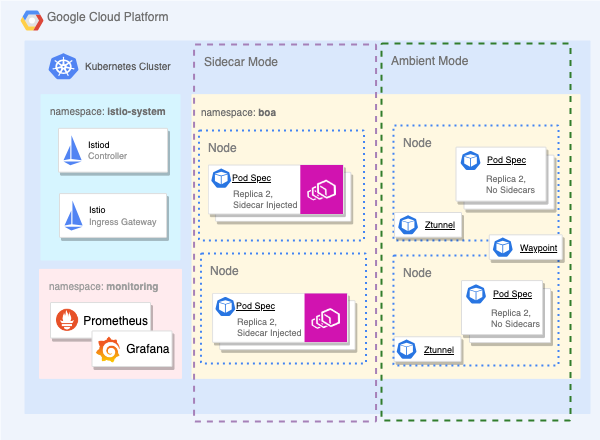
\includegraphics[width=1.0\linewidth]{resources/single-ns-test-infra.drawio.png}
    \caption{GCP Infrastructure Architecture with Single Namespace}
    \label{method:singleNsInfraArch}
\end{figure}

On the other hand, Figure \ref{method:multiNsInfraArch} shows the GCP infrastructure visualization of multiple namespace deployment (\cite{multiNsArticle}) of \acrshort{boa} application. The diagram shows up to 3 namespace deployment to keep the complexity of the figure lower however in the actual test 8 namespaces are used, each namespace representing a single microservice. In multiple namespace deployment environment, 'istio-system' and 'monitoring' namespaces remain unchanged but the data plane components of Istio are changed marginally. A Ztunnel is deployed per node wise whereas instance of Waypoint proxy is seen multiple times to cover multiple namespaces.
\begin{figure}[ht!]
    \centering
    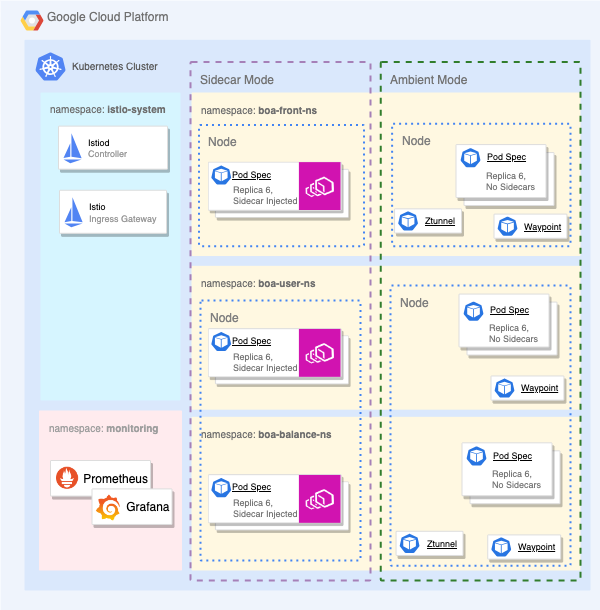
\includegraphics[width=1.0\linewidth]{resources/multi-ns-test-infra.drawio.png}
    \caption{GCP Infrastructure Architecture with Multiple Namespaces}
    \label{method:multiNsInfraArch}
\end{figure}


\subsubsection{Operational Complexity Measurement}
On a live Kubernetes cluster with hundreds or thousands of microservices, upgrading Istio becomes a challenge. Istio upgrades are important to avoid any vulnerabilities hence Istio documentation (\cite{istioDocCanaryUpgrade}) recommends a safe way of upgrading by using blue-green and canary deployment strategies to roll out new versions. Even though these methods are used pod restart is inevitable as the sidecar does not upgrade when the injector is upgraded rather, all injected pods must be restarted for their sidecars to upgrade. Hence a multiple Istio version deployment is made side by side by using Istio revision and tagging features (\cite{postaIstio2021}). By this not only the pods can switch to Istio versions dynamically with a restart, the ingress gateways can also be switched with zero downtime. To achieve the desired blue-green deployment a Kubernetes load balancer is used and Istio ingress gateway service types are set to ClusterIP to avoid creating further load balancer services.

\begin{figure}[ht!]
  \centering
  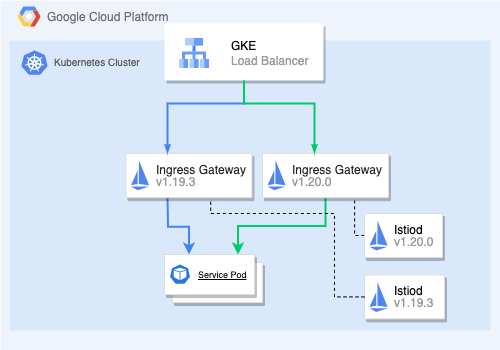
\includegraphics[width=1.0\linewidth]{resources/istio-upgrade-strategy.drawio.png}
  \caption{GCP Infrastructure Architecture of Istio Upgrade}
  \label{method:istioUpgradeArch}
\end{figure}

The upgrade architecture shown in Figure \ref{method:istioUpgradeArch} is heavily dependent on Istio Canary Deployment feature (\cite{istioDocHelm}). Istio version 1.18.5 is used a stable or blue version whereas version 1.19.3 is used as green version. Istio operator installation method is chosen for this test as it provides a greater control over parallel deployment instances of Istio.

Further to the Istio upgrade test, a no mesh to service mesh transition is also tested. When Istio is installed post application deployment on a Kubernetes cluster a restart of deployment is required for each namespaces. In sidecar mode, a Kubernetes object MutatingWebHookConfig acting as a webhook (\cite{krochmalski2017docker}) is deployed during Istio installation to track application pod creation and then to enable Istiod to inject a sidecar. All these pod detection and sidecar injection happens during pod initialization phase, hence if the Istio is installed after an application deployment Kubernetes admins always struggles to add Istio in the existing services. Fortunately, most of the times this is not a concern as in enterprise level, applications are deployed only after Kubernetes cluster is configured and validated with required elements including Istio. For academic purposes, this test checks whether ambient mode clears this blockers for cluster admins.

\subsection{Test Readiness}
\label{testReadiness}
Istio remains the core part of this research and to produce the research report on ambient mesh this paper explores the performance and operational complexity of Istio ambient mode. However, to test Istio from a real life cloud deployment environment, a deep dive into demo application deployment, Istio configuration and verification is required for a successful research result. In this section how Istio is installed, configured and verified is discussed along with \acrshort{boa} application set.

Istio documentation (\cite{istioDocInstall}) refers different methods for installing Istio system on a Kubernetes cluster however the preferred way is to use Istioctl - a tool which is installed on local system and uses Helm charts internally to install Istio on remote Kubernetes cluster. However for the Istio upgrade test the direct helm chart method is used in this research to use blue-green deployment. Istioctl comes with a lot of additional benefits like quick deployment of an ingress gateway or monitoring tool installation for testing purposes. In this research, Istio is installed and uninstalled several times using Istioctl and Helm Charts to capture test results. While using Istioctl, mainly two predefined profiles 'default' and 'ambient' is passed as command line argument to install Istio on remote cluster. A clean installation of Istio brings up two core components of Istio, Istiod - the control plane and the ingress controller in 'istio-system' namespace. These remains valid for both sidecar and ambient modes without any differences. Figure \ref{method:istioStdInstalledView} shows the cluster pod view from K9S - a tool used in all the tests to verify and query Kubernetes cluster components.

\begin{figure}[ht!]
    \centering
    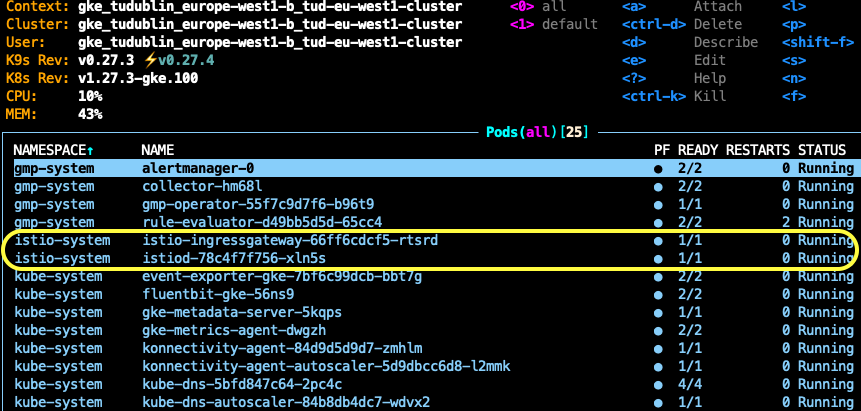
\includegraphics[width=1.0\linewidth]{resources/istio-std-installed.png}
    \caption{K9S View of Istio Control Plane}
    \label{method:istioStdInstalledView}
\end{figure}

The ingress gateway is used to serve the frontend microservice over public IP address whereas the Istiod configures all the sidecar proxies, Ztunnels and Waypoint proxies wherever these are application. 

A load testing script written in Python with Locust framework (\cite{locustDoc}) is used which comes by default as a microservice with \acrshort{boa} project. However, for this research project, some parameters of the script is modified and used from local test machine to simulate the live traffic to \acrshort{boa} application. With each tests, 50 user traffic is simulated at a rate of 1 per second for 10 minutes to perform sign up, login, transaction and logout operations.

\begin{figure}[ht!]
  \centering
  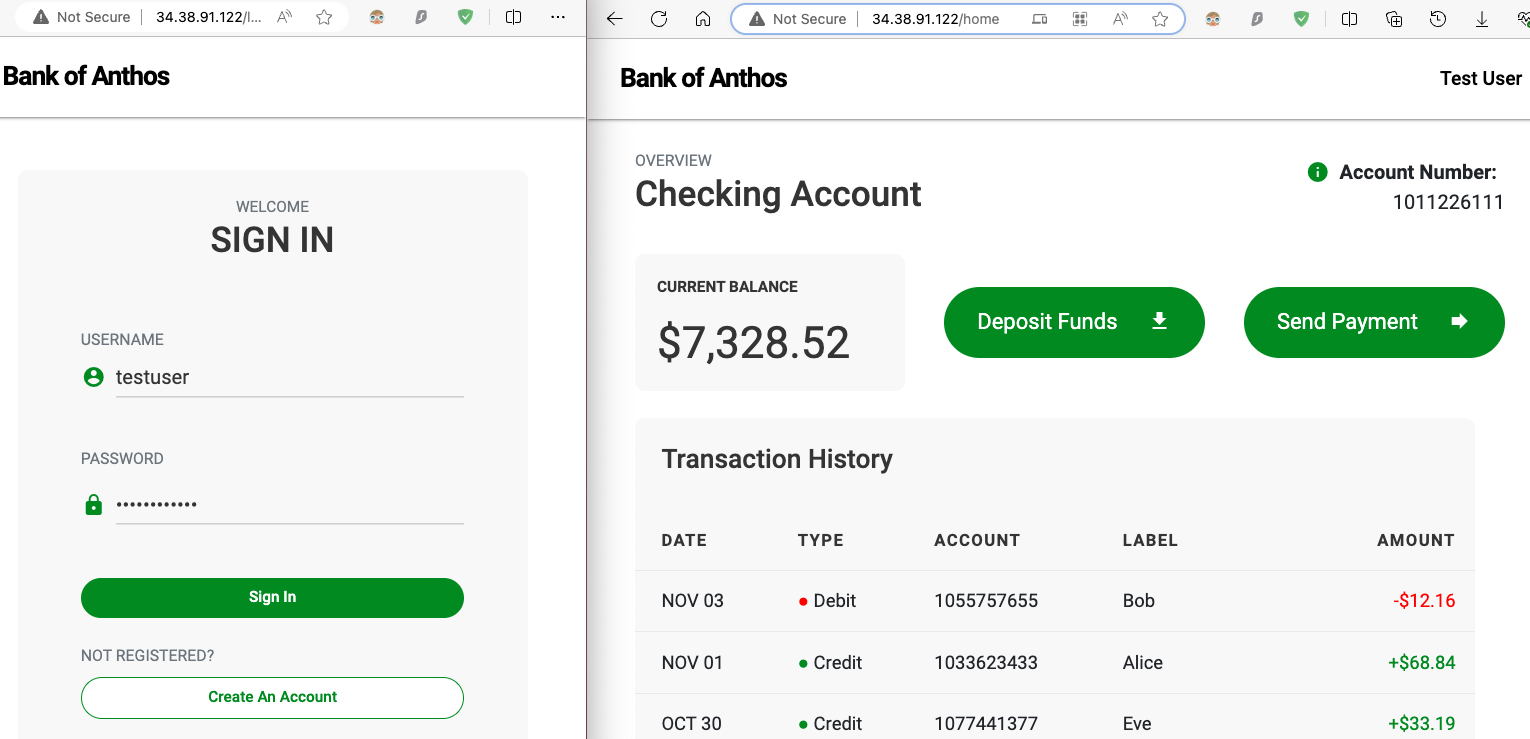
\includegraphics[width=1.0\linewidth]{resources/boa-view.png}
  \caption{Bank-of-anthos is accessible over external load balancer}
  \label{method:boaWebView}
\end{figure}

Figure \ref{method:boaWebView} shows the frontend view of the \acrshort{boa} application when it is accessed over public IP address. For some small test verifications a manual UI navigation method is also used by navigating to different pages of \acrshort{boa}.


\subsubsection{Sidecar Mode Test Setup}
With the \acrshort{gke} cluster in place and the Istio system installed with Istioctl 'default' profile, istiod - the control plane and an ingress gateway controller is deployed to the 'istio-system' namespace. An application namespace 'boa' is created for single namespace deployment test and 8 different namespaces are created by the microservice manifest files in case of multiple namespace deployment scenario. Namespace labelling is done with 'istio-injection=enabled' to configure the Istio control plane for injecting sidecars into microservice pods. For the \acrshort{boa} application deployment, first the JSON web token is deployed to 'boa' namespace as a ConfigMap followed by applying microservice manifests files. Accounts DB and Ledger DB microservices are deployed as StatefulSet whereas rest of the microservices are deployed as Kubernetes Deployment object. Once everything is successfully deployed, the K9s view shows all microservice pods with two replicas each in case of single namespace deployment and six replicas in case of multiple namespace deployment. As part of the verification process the pod descriptions are checked using K9s which reveals the sidecar container as 'istio-proxy' as shown in Figure \ref{method:istioSidecarInjectionView}.

\begin{figure}[ht!]
  \centering
  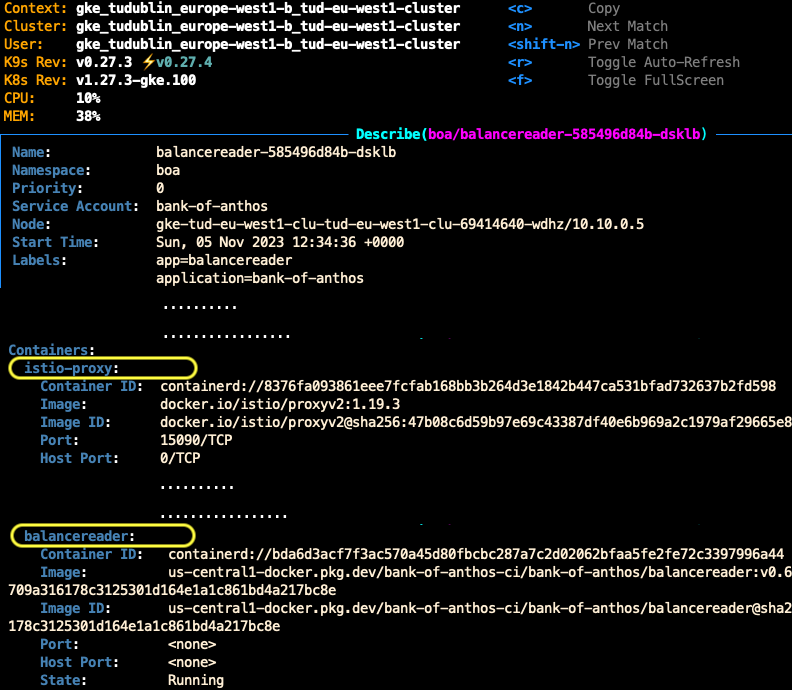
\includegraphics[width=1.0\linewidth]{resources/istio-sidecar-injection.png}
  \caption{Istio sidecar injection is in action}
  \label{method:istioSidecarInjectionView}
\end{figure}

In order to access the frontend microservice over a public IP address, a frontend gateway is attached to the istio ingress controller. By browsing to external IP address of the istio ingress controller, the \acrshort{boa} application is accessible from local system which confirms the application deployment. At this point, a verification is done whether Istio data plane is engaged in offering the basic service mesh functionality like mTLS encryption. Wireshark, a well known tool for packet sniffing is used on local system with kubectl plugin ksniff to intercept network packets between 2 microservices, frontend and balance reader. This verification involves a two stage process where the microservices are deployed previously on the cluster without Istio and the current deployment with Istio sidecar mode. While comparing the Wireshark captures for both cases, a balance value of "71580" is shown in plain text in case of no mesh set up. The plain text value is shown in Figure \ref{method:plainTxtWiresharkView} when Istio is not deployed.

\begin{figure}[ht!]
  \centering
  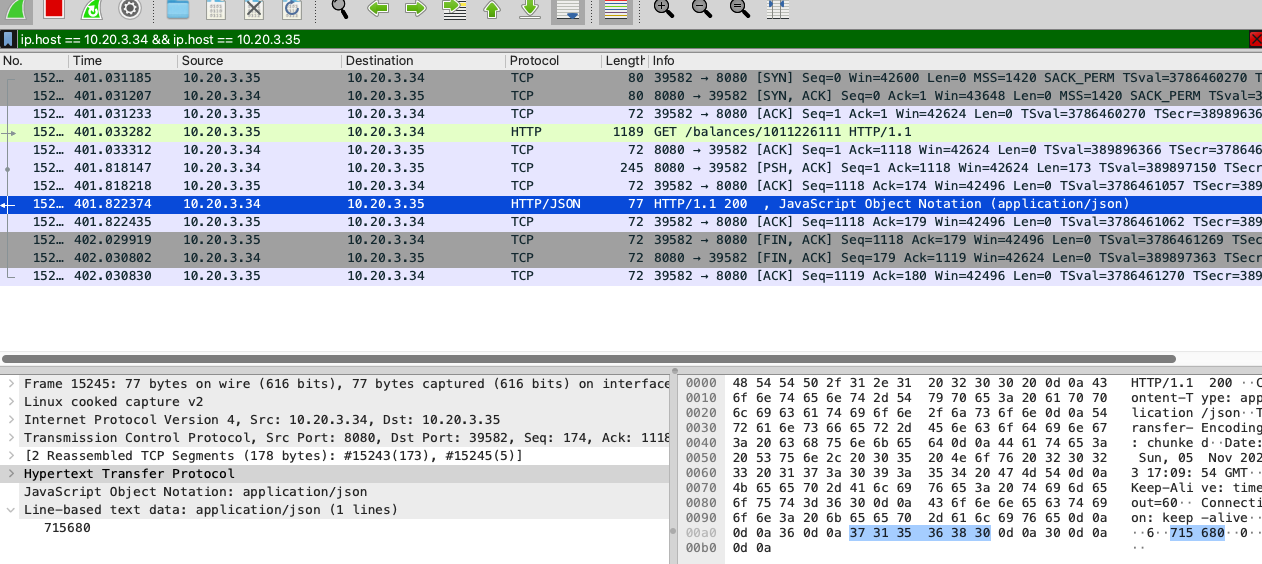
\includegraphics[width=1.0\linewidth]{resources/raw-balance-value.png}
  \caption{Plain Text Inter-Service Communication in No-Mesh Mode}
  \label{method:plainTxtWiresharkView}
\end{figure}

In single namespace test environment, 16 pods are running where:
\begin{itemize}
  \item Two replicas of eight microservices running a total of 16 sidecars
  \item Three cluster nodes are used to host 16 pods
\end{itemize}

In multiple namespace test environment the pod counts are 48 where:
\begin{itemize}
  \item Six replicas of eight microservices running 48 sidecars
  \item Eight cluster nodes are used to host 48 pods
\end{itemize}


\subsubsection{Ambient Mode Test Setup}
Ambient mode of Istio is installed using Istioctl, similar to sidecar mode but with a different profile named 'ambient'. This installation creates the istio-system namespace and deploys istiod control plane along with CNI plugin. Once the Istiod control plane is provisioned it spawns Ztunnel proxy pods on each running nodes. An Ingress controller is also used here and the frontend gateway is attached to it. The process of namespace labelling remains same but with a different key value pair of "istio.io/dataplane-mode=ambient". Though the majority of set up process remains same like sidecar mode, the verification process is different. To check the Ztunnel engagement, a handful traffic is sent to \acrshort{boa} by using the load generator script and packet sniffing is done for one of the microservice pod and a Ztunnel pod. The following two figures shows how the traffic is first intercepted by Ztunnel and then passed to the microservice pod. A closer look to Figure \ref{method:ztunnelLogView} and \ref{method:ztunnelTraceView} shows that Ztunnel received the traffic from ingress gateway 10.20.0.22 and then passing to the respective service pods.

\begin{figure}[ht!]
  \centering
  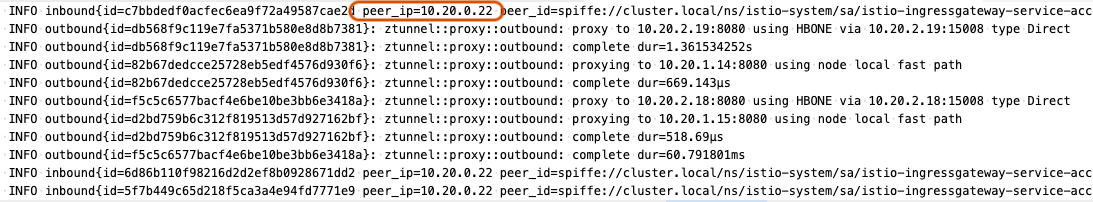
\includegraphics[width=1.0\linewidth]{resources/ztunnel-log.png}
  \caption{Ztunnel Pod Receiving Traffic}
  \label{method:ztunnelLogView}
\end{figure}

\begin{figure}[ht!]
  \centering
  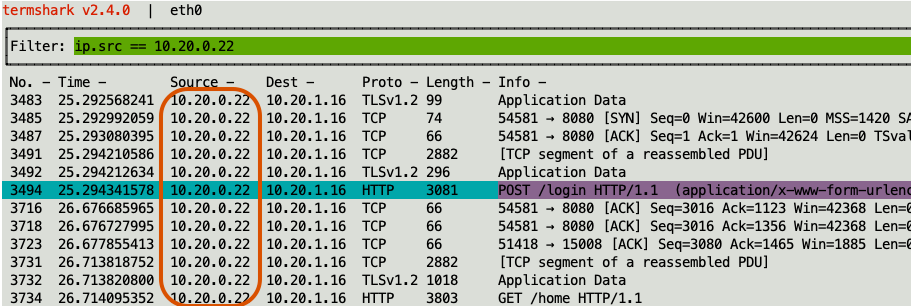
\includegraphics[width=1.0\linewidth]{resources/ztunnel-network-trace.png}
  \caption{Ztunnel Forwards Traffic to Microservice Pod}
  \label{method:ztunnelTraceView}
\end{figure}

To install the layer 7 proxy Waypoint Kubernetes gateway API CRDs are required to be installed on cluster as by default CRDs are not available with Istio installation. After configuring the custom CRDs required for Waypoint, each namespace gets a Waypoint proxy pod. When all microservices are deployed in a single namespace mapped there get a single Waypoint proxy but when the microservices are deployed across multiple namespaces, Waypoint proxies are deployed to each one of them. A comparison between Waypoint proxies deployed in single and multiple namespaces remains a crucial part of this research as it illustrates some most common real life deployment scenario where microservices are deployed in different namespaces. Figure \ref{method:waypointAppliedView} shows how the Waypoint proxy is engaged in ambient mesh setup to the microservice pods.

\begin{figure}[ht!]
  \centering
  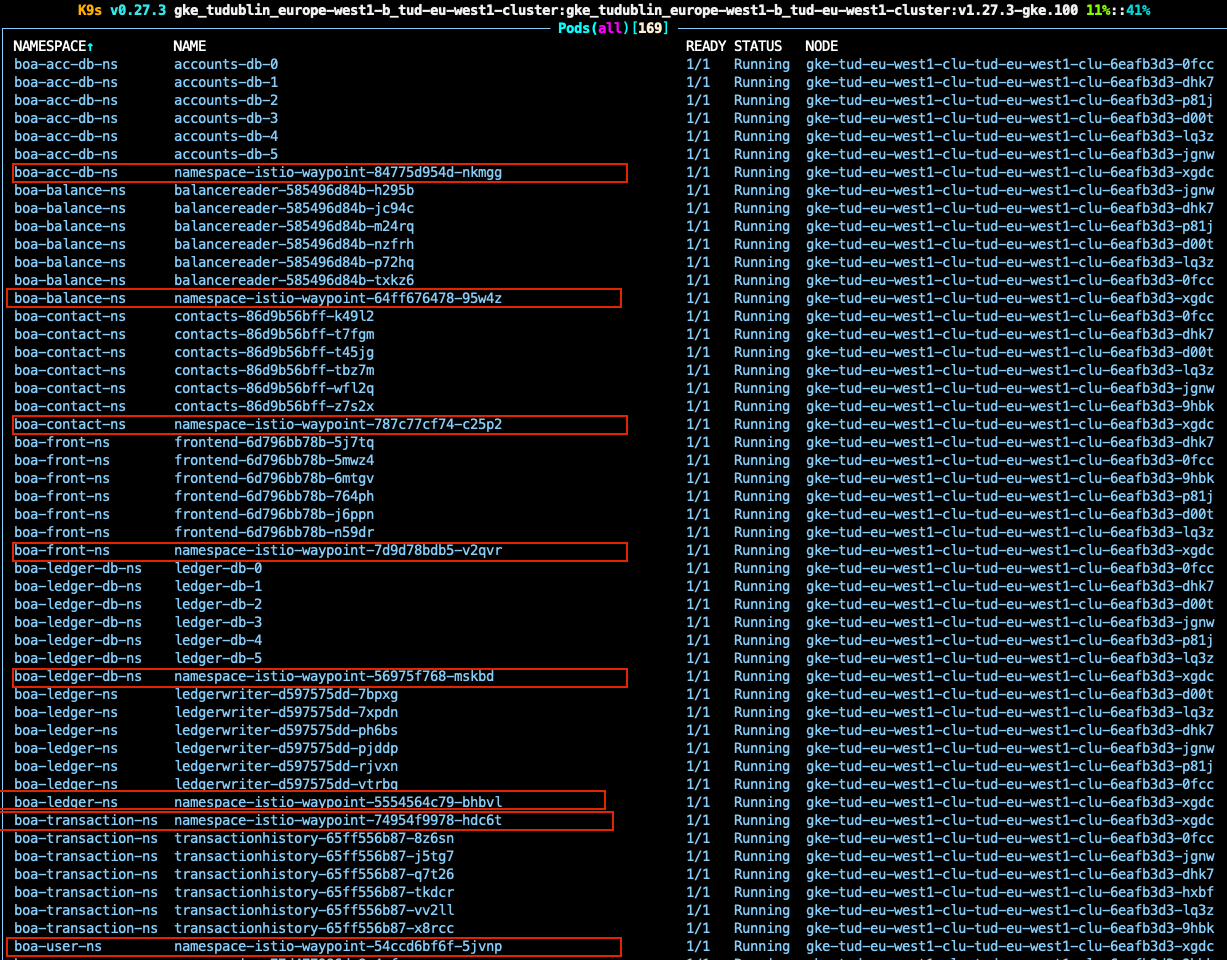
\includegraphics[width=1.0\linewidth]{resources/ambient-multi-ns-l4-l7-deployed.png}
  \caption{Waypoint Proxy is Applied Per Namespace Wise}
  \label{method:waypointAppliedView}
\end{figure}

To engagement Waypoint proxy, a L7 policy (Appendix \ref{appendix:waypoint}) is applied to return a direct response from the balance reader microservice. For the research purpose a simple HTTP filtering is done based on the host name where all the requests made to balance reader microservice will result in a HTTP 503 error. The L7 policy is applied via a Kubernetes manifest file and it is targeted to application namespace. Multiple namespace test scenario applies this policy to the balance reader namespace only. As the frontend is not able to get the balance value from balance reader microservice a '---' is displayed as shown in Figure \ref{method:l7PolicyAppliedView} when accessing \acrshort{boa} from a browser. This implies the traffic flows from istio ingress to host level Ztunnel proxy and finally followed by the Waypoint proxy before reaching to balance reader microservice.
To see Waypoint proxy engagement, a L7 policy (Appendix \ref{appendix:waypoint}) is applied to return a direct response from the balance reader microservice. For the research purpose a simple HTTP filtering is done based on the host name where all the requests made to balance reader microservice will result in a HTTP 503 error. The L7 policy is applied via a Kubernetes manifest file and it is targeted to application namespace. Multiple namespace test scenario applies this policy to the balance reader namespace only. As the frontend is not able to get the balance value from balance reader microservice a '---' is displayed as shown in Figure \ref{method:l7PolicyAppliedView} when accessing \acrshort{boa} from a browser. This implies the traffic flows from istio ingress to host level Ztunnel proxy and finally to Waypoint proxy before reaching to balance reader microservice.

\begin{figure}[ht!]
  \centering
  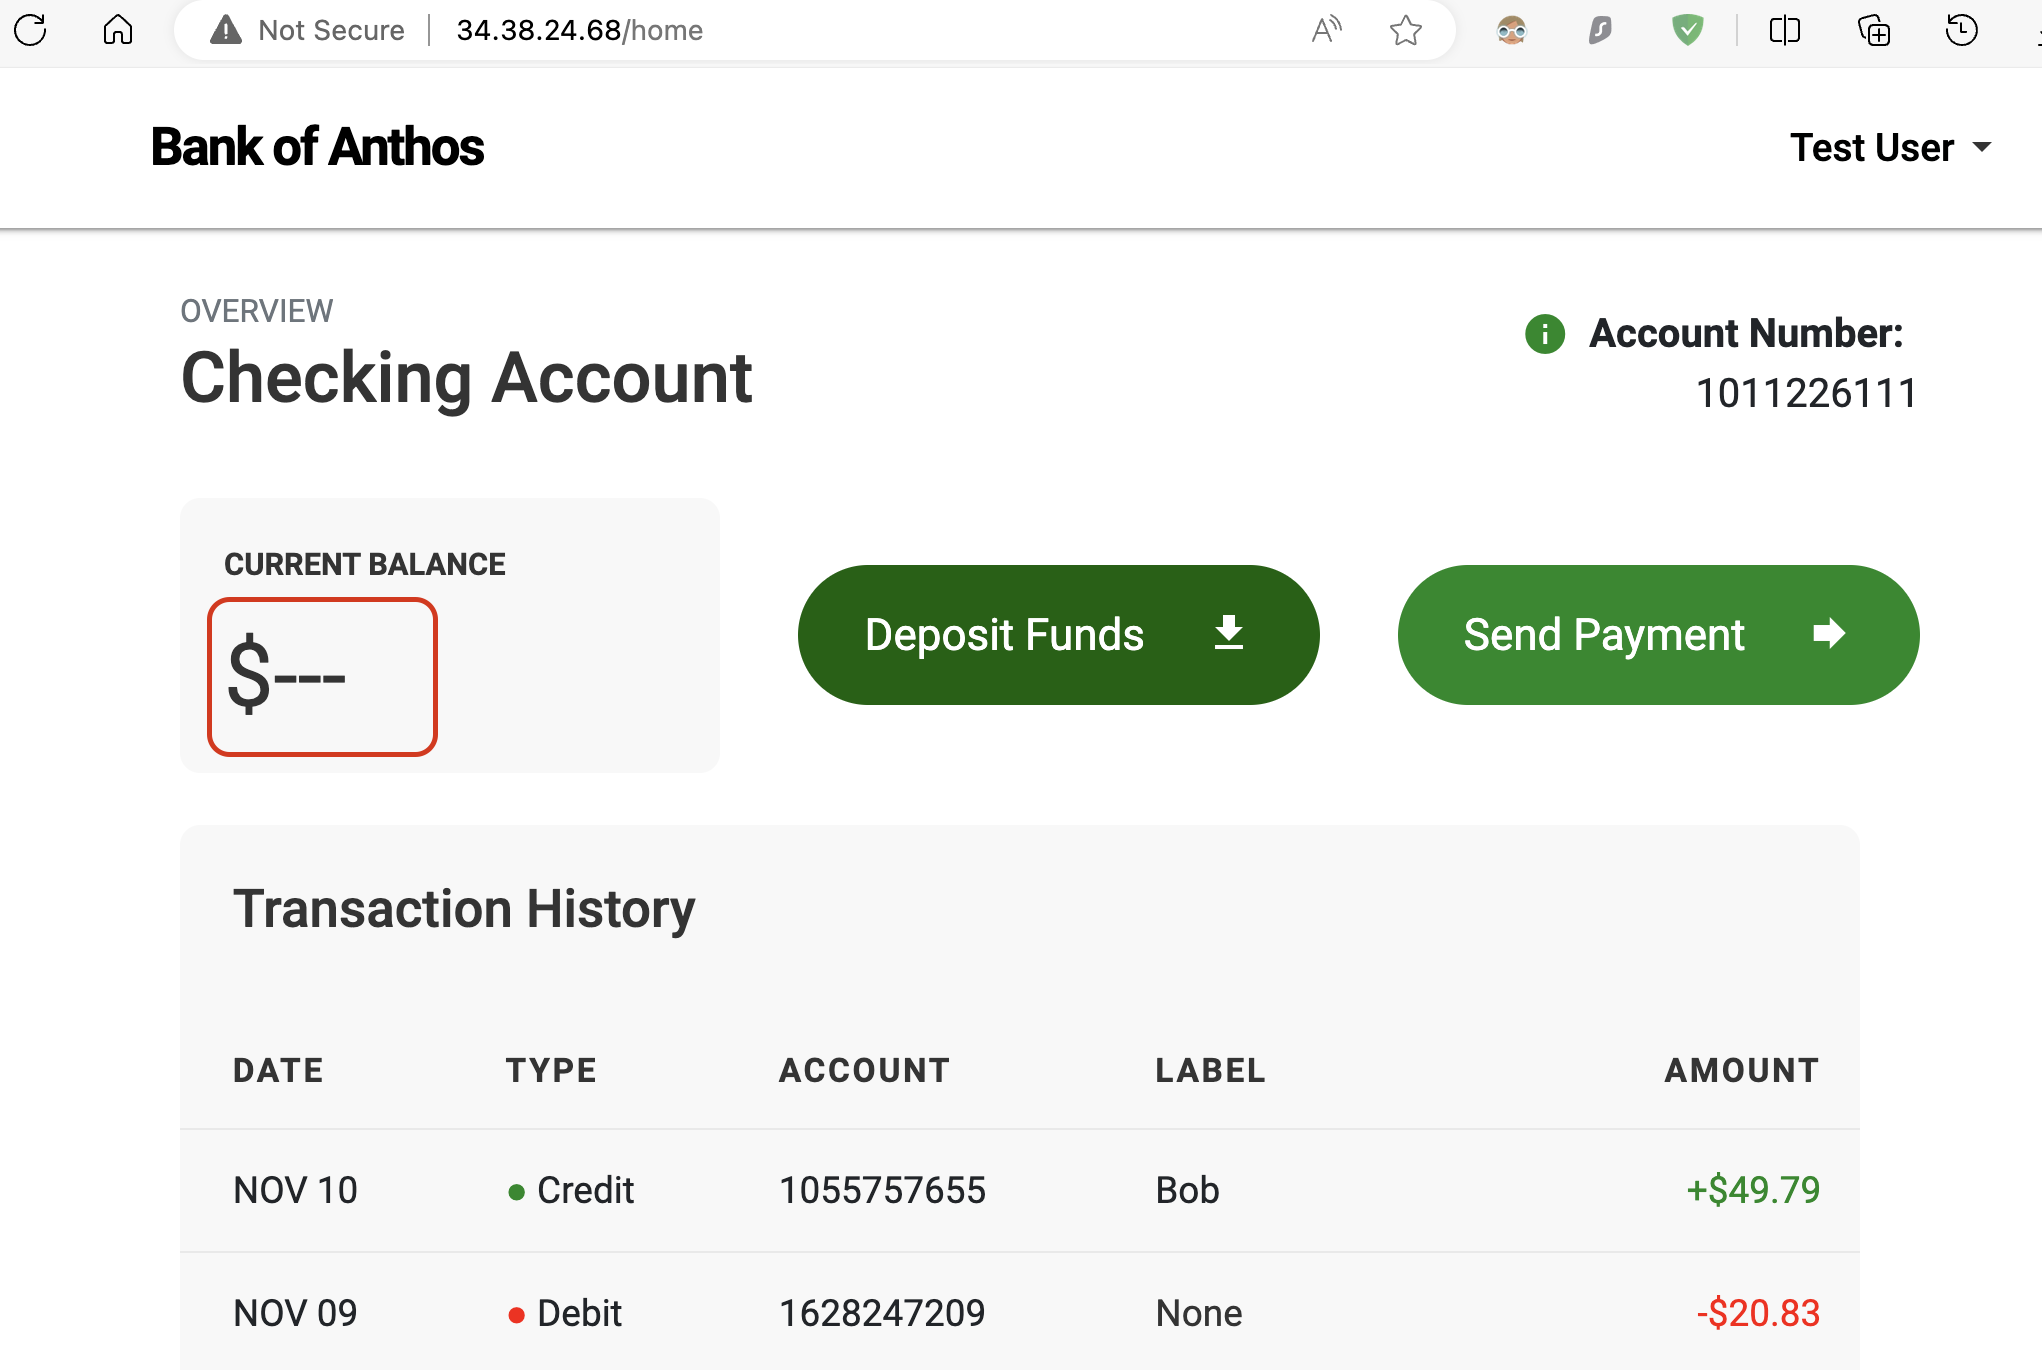
\includegraphics[width=0.7\linewidth]{resources/l7-policy-applied.png}
  \caption{Waypoint L7 Policy Reflecting on Frontend}
  \label{method:l7PolicyAppliedView}
\end{figure}

In single namespace test environment the pod count is 16 where:
\begin{itemize}
  \item Two replicas of eight microservices running without any sidecars
  \item Two Ztunnel proxy pods on 2 nodes
  \item One Waypoint proxy pod in the single namespace
\end{itemize}

In multiple namespace test environment the pod count is 48 where:
\begin{itemize}
  \item Six replicas of eight microservices without any sidecars
  \item Nine cluster nodes are used to host 48 pods
  \item Eight Waypoint proxy pods are deployed in 8 namespaces to support L7 processing
\end{itemize}

\subsubsection{Istio Upgrade Test Setup}
For Istio upgrade a different strategy is applied than testing Istio for performance benchmarking. The process involves deploying Istio operator - a program in the cluster to manage the state of Istio deployments. Istio operator manifest files come by default with Istioctl package but a custom resource definition or operator specification is made to configure the Istio control plane deployment. To deploy multiple versions of Istio on the same cluster, each version of Istioctl needs to be downloaded on the local system. The helm chart manifest files are applied to the cluster using 'kubectl' to deploy the operator. Once the operator is live on the cluster, the operator specification is applied to setup the Istiod control plane. This specification defines the Istio profiles to be installed on the cluster, which is 'minimal' and 'ambient' for sidecar and ambient mode respectively. By default the operator specification deploys an ingress gateway as well but that is restricted in the configuration to create manually in next stage. To verify the Istiod deployment state and whether multiple versions are running side by side on the cluster a kubectl describe pod command is used as shown in Figure \ref{method:multiIstiodVersions}.

\begin{figure}[ht!]
  \centering
  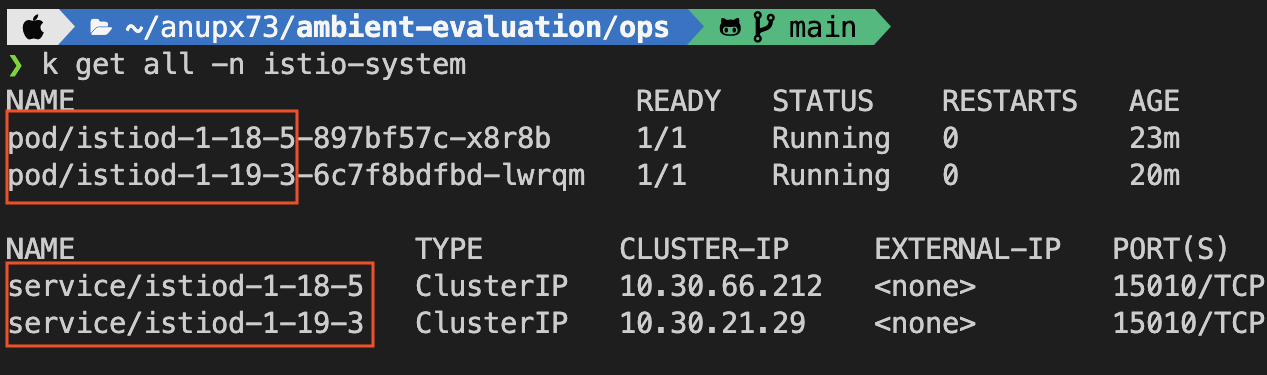
\includegraphics[width=1.0\linewidth]{resources/multi-istiod.png}
  \caption{Multiple Versions of Istiod is Live on Cluster}
  \label{method:multiIstiodVersions}
\end{figure}

Similarly, the ingress gateways are also deployed to the cluster with a defined configuration (Appendix \ref{appendix:researchRepo}) where the service type is set to ClusterIP to enable the ingress gateway service to maintain a local cluster IP address. As shown in Figure \ref{method:multiGateways} two Istio gateways are operating with different revisions and one of them are selected by the external Kubernetes load balancer to route the traffic.

\begin{figure}[ht!]
  \centering
  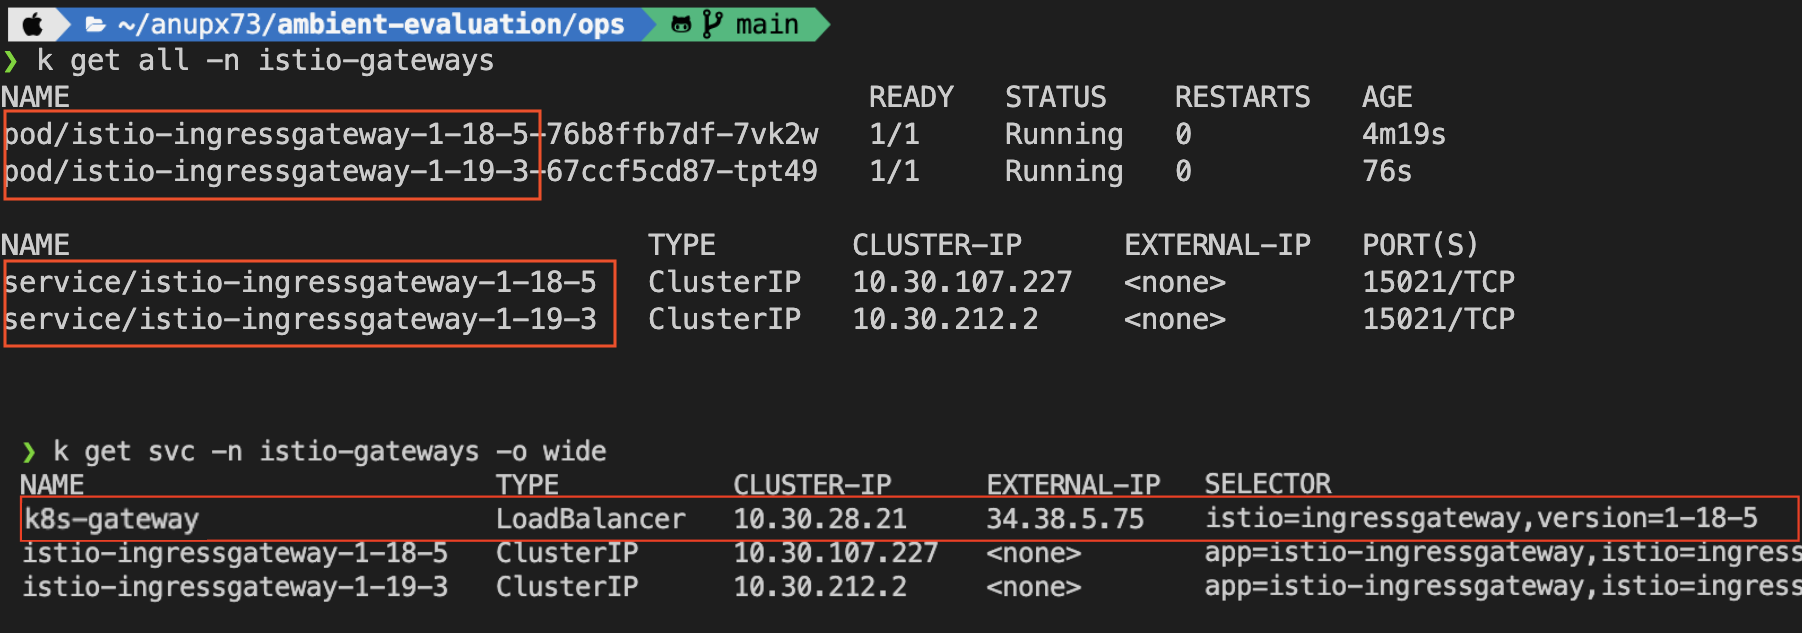
\includegraphics[width=1.0\linewidth]{resources/multi-gateways.png}
  \caption{Multiple Versions of Ingress Gateways and Load Balancer}
  \label{method:multiGateways}
\end{figure}

\subsection{Challenges Encountered}
\subsubsection{Ztunnel Blocks Service Start}
While setting up Istio with ambient mode, couple of microservices pods were stuck in Running state till the Ztunnel pod on the specific node was restarted. The configuration was:

\begin{itemize}
\item Istio with ambient profile installed on 3 nodes
\item 1 replica of all 8 microservices were deployed to a single node
\item Microservice deployment was done post Istio installation and namespace labelling
\end{itemize}

This scenario was not reproducible quite often, but this may need a further investigations into application configuration before flagging as a ambient mesh.

\subsubsection{Grafana Cloud Integration}
Grafana Cloud was chosen at first as a monitoring platform to retain research test data for a long period of time. After the Grafana cloud integration with the GKE instance was made, a few tests were done with Istio system data capture. This resulted in exceeding the free-tier metric limit of 10000 per month by 400\%. Later, the metric ingestion limit was controlled up to a certain limit by adding a filter in the Prometheus remote data export configuration; however, to avoid any unforeseen issues, switching to a Grafana local instance was preferred. Appendix \ref{appendix:grafana} mentions the details about setting up Grafana cloud integration.
\pagebreak


\section{Results}
\label{resultSection}
\subsection{Compute Resource Utilization}
Section \ref{testReadiness} describes how Istio system resource utilization comparison test is designed with two different environments - single and multiple namespace deployment. In this section test result data and graphs are presented from Grafana with a minimum, maximum and a mean value of CPU and memory consumption over a ten minutes time period for each test. Though the test target is to compare Istio system resource utilization between sidecar and ambient modes, looking at a microservice pod resource utilization in first place gives some intial impression of ambient mode memory efficiency.

\begin{figure}[ht!]
  \centering
  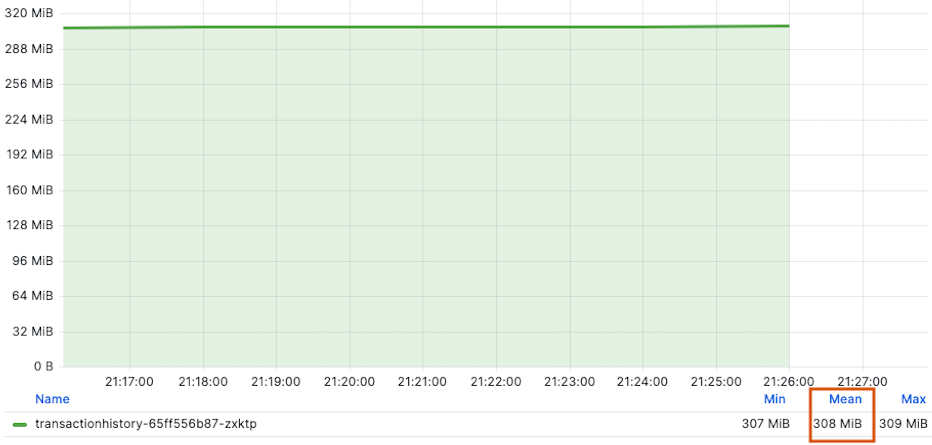
\includegraphics[width=0.73\linewidth]{resources/sidecar-pod-mem.png}
  \caption{Pod Memory Use in Sidecar Mode}
  \label{result:podMemUseSidecar}
\end{figure}

\begin{figure}[ht!]
  \centering
  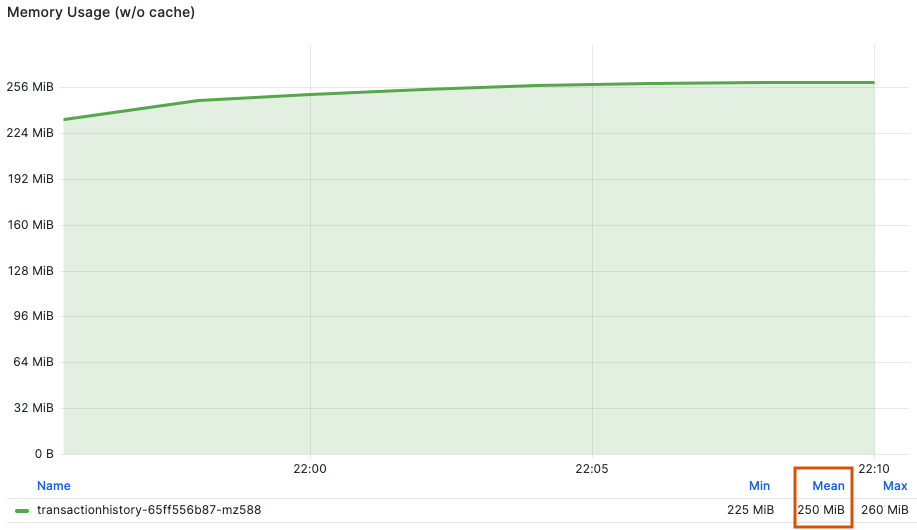
\includegraphics[width=0.73\linewidth]{resources/ambient-pod-mem.png}
  \caption{Pod Memory Use in Ambient L4 Processing Mode}
  \label{result:podMemUseAmbient}
\end{figure}

Figure \ref{result:podMemUseSidecar} and \ref{result:podMemUseAmbient} shows two ten minutes memory usage graph of transaction history microservice pods captured from a single namespace test environment. Looking at the mean or average value of memory usage a significant difference is notice. In sidecar mode the average memory usage is 308 \gls{mib} whereas in ambient mode with L4 processing layer its only 250 \gls{mib}. This result interprets an improvement of 23.2\% memory usage in ambient mode however while comparing the CPU usage there is no noticable difference found hence the CPU usage details are not shown here. Rest of this section presents the test result graphs from twelve different test cases covering both single and multiple namespace environments. Looking at the graph and test values from bottom right side of the graphics can be intimidating hence before discussing further, Table \ref{allCpuResultsTable} and \ref{allMemResultsTable} summarizes the test results in tabular form. Both the table shows a raw data captured from Grafana with decimal point limited maximum to three places for both CPU and memory utilization.

\begin{table}[ht!]
  \centering
  \begin{tabular}{ |l|c|c|c|c|}
    \hline
    \textbf{Test Environment} & \textbf{\textit{Istio Mode}} & \textbf{\textit{Min}} & \textbf{\textit{Mean}} & \textbf{\textit{Max}} \\
    \textbf{\textit{ }} & \textbf{\textit{ }} & \textbf{\textit{(vCPU)}} & \textbf{\textit{(vCPU)}} & \textbf{\textit{(vCPU)}} \\ \hline
    Single Namespace & Sidecar & 0.020 & 0.107 & 0.125 \\ \hline
    Single Namespace & Ambient L4 & 0.020 & 0.052 & 0.065 \\ \hline
    Single Namespace & Ambient L4+L7 & 0.058 & 0.099 & 0.116 \\ \hline

    Multiple Namespace & Sidecar & 0.230 & 0.403 & 0.463 \\ \hline
    Multiple Namespace & Ambient L4 & 0.075 & 0.208 & 0.235 \\ \hline
    Multiple Namespace & Ambient L4+L7 & 0.124 & 0.245 & 0.344 \\ \hline
  \end{tabular}
  \caption{CPU Usage of Istio System in Different Test Environments}
  \label{allCpuResultsTable}
\end{table}

\begin{table}[ht!]
  \centering
  \begin{tabular}{ |l|c|c|c|c|}
    \hline
    \textbf{Test Environment} & \textbf{\textit{Istio Mode}} & \textbf{\textit{Min}} & \textbf{\textit{Mean}} & \textbf{\textit{Max}} \\
    \textbf{\textit{ }} & \textbf{\textit{ }} & \textbf{\textit{(MiB)}} & \textbf{\textit{(MiB)}} & \textbf{\textit{(MiB)}} \\ \hline
    Single Namespace & Sidecar & 321 & 582 & 610 \\ \hline
    Single Namespace & Ambient L4 & 52.0 & 67.3 & 70.3 \\ \hline
    Single Namespace & Ambient L4 + L7 & 107 & 120 & 124 \\ \hline
    
    Multiple Namespace & Sidecar & 1822.72 & 1843.2 & 1889.68 \\ \hline
    Multiple Namespace & Ambient L4 & 62.4 & 88.6 & 94.5 \\ \hline
    Multiple Namespace & Ambient L4 + L7 & 387 & 461 & 608 \\ \hline
  \end{tabular}
  \caption{Memory Usage of Istio System in Different Test Environments}
  \label{allMemResultsTable}
\end{table}


%%single ns
%sidecar cpu, mem
\begin{figure}[H]
  \centering
  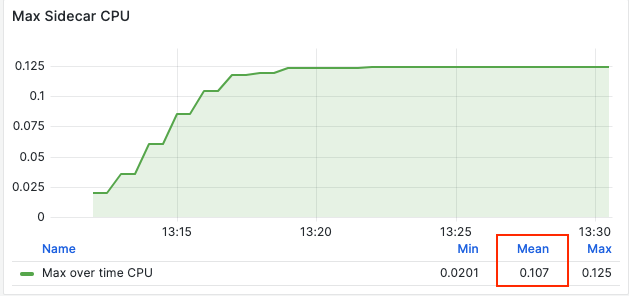
\includegraphics[width=0.8\linewidth]{resources/max-sidecar-cpu.png}
  \caption{CPU Usage of Sidecar Mode in Single Namespace}
\end{figure}

\begin{figure}[H]
  \centering
  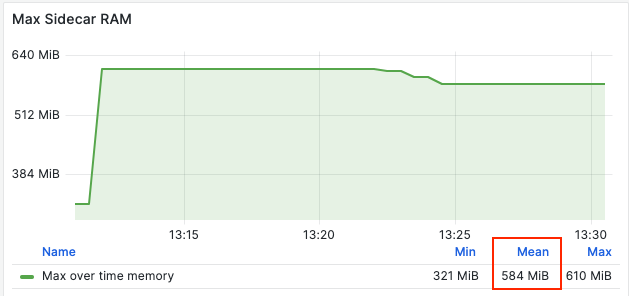
\includegraphics[width=0.8\linewidth]{resources/max-sidecar-mem.png}
  \caption{Memory Usage of Sidecar Mode in Single Namespace}
\end{figure}

%ambient l4 cpu, mem
\begin{figure}[H]
  \centering
  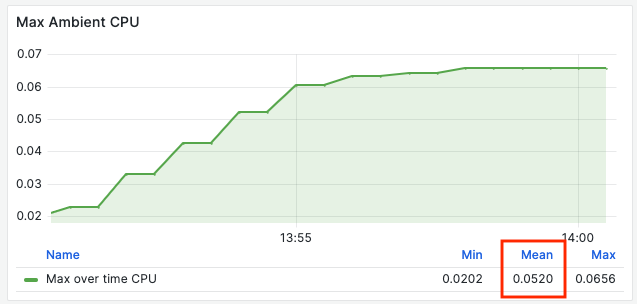
\includegraphics[width=0.8\linewidth]{resources/max-ambient-l4-cpu.png}
  \caption{CPU Usage of Ambient Mode(L4 Only) in Single Namespace}
\end{figure}

\begin{figure}[H]
  \centering
  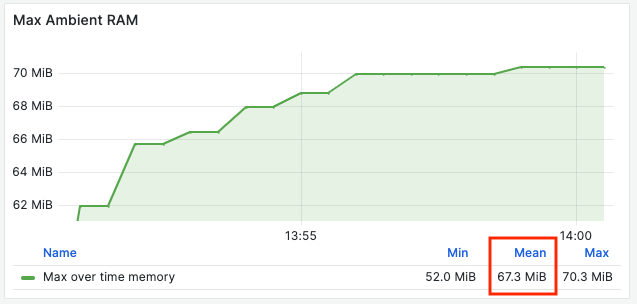
\includegraphics[width=0.8\linewidth]{resources/max-ambient-l4-mem.png}
  \caption{Memory Usage of Ambient Mode(L4 Only) in Single Namespace}
\end{figure}

%ambient l4+l7 cpu, mem
\begin{figure}[H]
  \centering
  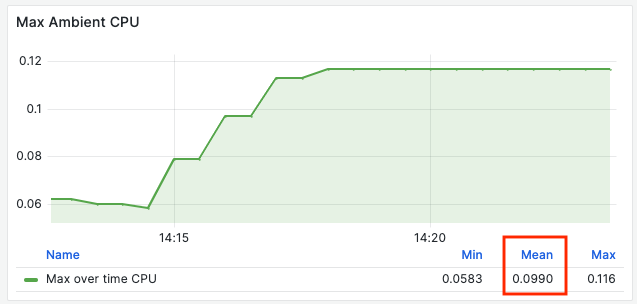
\includegraphics[width=0.78\linewidth]{resources/max-ambient-l4-l7-cpu.png}
  \caption{CPU Usage of Ambient Mode(L4 + L7) in Single Namespace}
\end{figure}

\begin{figure}[H]
  \centering
  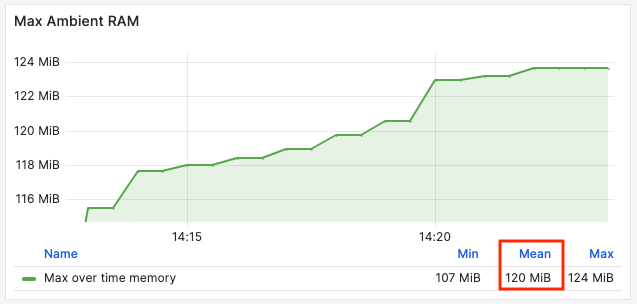
\includegraphics[width=0.8\linewidth]{resources/max-ambient-l4-l7-mem.png}
  \caption{Memory Usage of Ambient Mode(L4 + L7) in Single Namespace}
\end{figure}


%%multi ns
%sidecar cpu, mem
\begin{figure}[H]
  \centering
  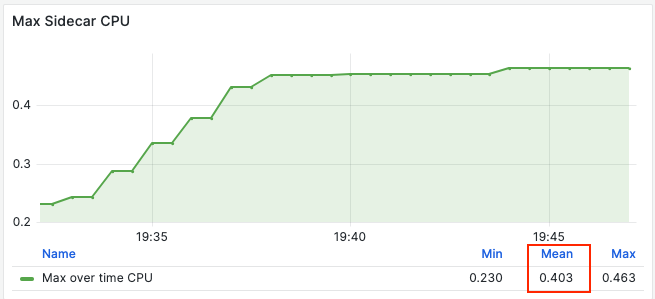
\includegraphics[width=0.8\linewidth]{resources/multi-ns-sidecar-cpu.png}
  \caption{CPU Usage of Sidecar Mode in Multiple Namespace}
\end{figure}

\begin{figure}[H]
  \centering
  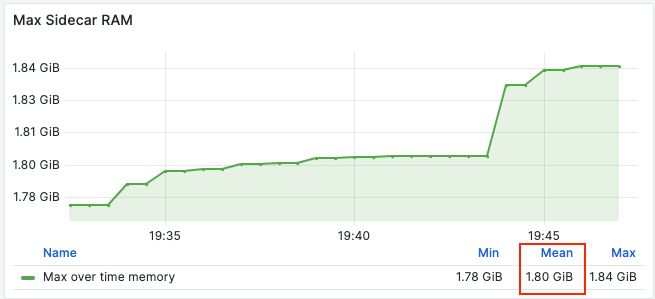
\includegraphics[width=0.8\linewidth]{resources/multi-ns-sidecar-mem.png}
  \caption{Memory Usage of Sidecar Mode in Multiple Namespace}
\end{figure}

%ambient l4 cpu, mem
\begin{figure}[H]
  \centering
  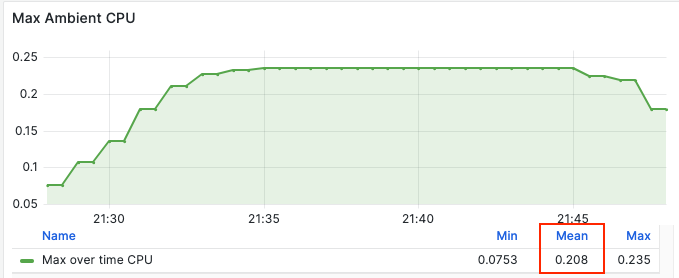
\includegraphics[width=0.8\linewidth]{resources/ambient-multi-ns-l4-cpu.png}
  \caption{CPU Usage of Ambient Mode(L4 Only) in Multiple Namespace}
\end{figure}

\begin{figure}[H]
  \centering
  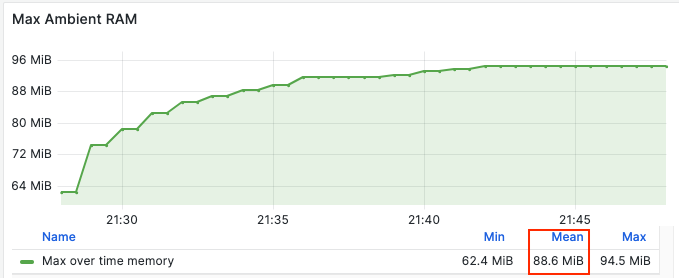
\includegraphics[width=0.85\linewidth]{resources/ambient-multi-ns-l4-mem.png}
  \caption{Memory Usage of Ambient Mode(L4 Only) in Multiple Namespace}
\end{figure}

%ambient l4+l7 cpu, mem
\begin{figure}[H]
  \centering
  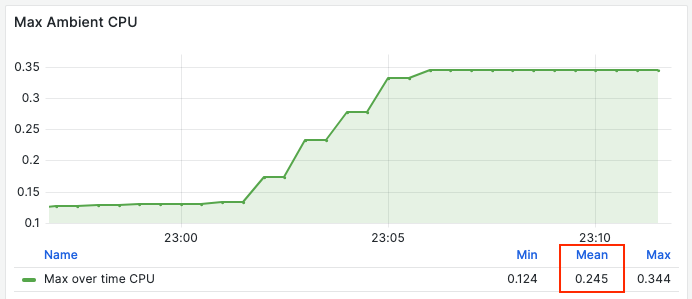
\includegraphics[width=0.85\linewidth]{resources/ambient-multi-ns-l4-l7-cpu.png}
  \caption{CPU Usage of Ambient Mode(L4 + L7) in Multiple Namespace}
\end{figure}

\begin{figure}[H]
  \centering
  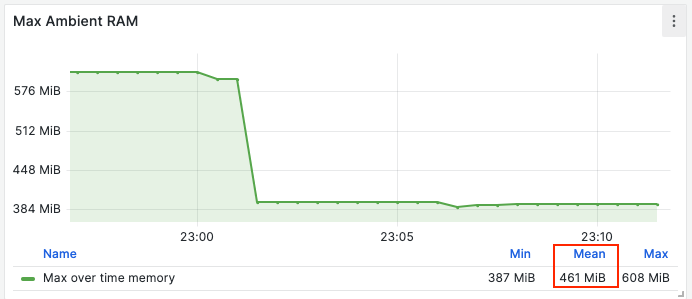
\includegraphics[width=0.85\linewidth]{resources/ambient-multi-ns-l4-l7-mem.png}
  \caption{Memory Usage of Ambient Mode(L4 + L7) in Multiple Namespace}
\end{figure}

With the above test results in place, lets find out the exact performance difference by comparing mean values of CPU and memory usage between sidecar mode, ambient mode with L4 proxy and ambient mode with L4 and L7 proxy. Two different comparison are done between sidecar mode and ambient mode with two different configurations to keep the Ztunnel and Waypoint proxy resource consumption tracked. Table \ref{sidecarCpuVsL4} shows an improvement of 51.4\% in CPU utilization from single namespace test scenario by using 0.107 vCPU by sidecar mode and 0.052 vCPU by ambient mode with L4 processing. In case of multiple namespace test scenario, the difference is 48\% where sidecar mode used 0.403 vCPU and ambient mode with L4 processing used only 0.208 vCPU. Table \ref{sidecarCpuVsL4L7} shows the difference between sidecar and ambient with L4 and L7 processing. The results are 7.4\% improvement in single namespace whereas 39\% improvement in multiple namespace test scenario.

\begin{table}[ht!]
  \centering
  \begin{tabular}{ |l|c|c|c| }
    \hline
    \textbf{Test Environment} & \textbf{\textit{Sidecar}} & \textbf{\textit{Ambient L4}} & \textbf{\textit{Improvement}}\\ \hline
    Single Namespace & 0.107 vCPU & 0.052 vCPU & 51.4\% \\ \hline
    Multiple Namespace & 0.403 vCPU & 0.208 vCPU & 48\% \\ \hline
  \end{tabular}
  \caption{\textit{CPU} Usage Comparison Between Sidecar and Ambient L4}
  \label{sidecarCpuVsL4}
\end{table}


\begin{table}[ht!]
  \centering
  \begin{tabular}{ |l|c|c|c| }
    \hline
    \textbf{Test Environment} & \textbf{\textit{Sidecar}} & \textbf{\textit{Ambient L4 + L7}} & \textbf{\textit{Improvement}}\\ \hline
    Single Namespace & 0.107 vCPU & 0.099 vCPU & 7.4\% \\ \hline
    Multiple Namespace & 0.403 vCPU & 0.245 & 39\% \\ \hline
  \end{tabular}
  \caption{\textit{CPU} Usage Comparison Between Sidecar and Ambient L4 + L7}
  \label{sidecarCpuVsL4L7}
\end{table}

Table \ref{sidecarMemVsL4} shows a side by side comparison of memory utilization between Istio sidecar mode and ambient mode with L4 proxy only followed by an improvement percentage. In single namespace environment, sidecar mode uses 584 MiB memory whereas in ambient mode the memory footprint is only 67.3 MiB translating an improvement of 88.47\% in memory usage. Similarly while comparing the results from multiple namespace test environment, the memory utilization is improved in ambient mode by 95.13\% from 1.8 GiB to only 88 MiB. Table \ref{sidecarMemVsL4L7} reflects the test comparison result between sidecar mode and ambient mode with both L4 and L7 processing. In single namespace test environment, the improvement is 79.45\% whereas in multiple namespace scenario the efficiency rate is 74.98\%.

\begin{table}[ht!]
  \centering
  \begin{tabular}{ |l|c|c|c| }
    \hline
    \textbf{Test Environment} & \textbf{\textit{Sidecar}} & \textbf{\textit{Ambient L4}} & \textbf{\textit{Improvement}}\\ \hline
    Single Namespace & 584 MiB & 67.3 MiB & 88.47\% \\ \hline
    Multiple Namespace & 1.8 GiB & 88.6 MiB & 95.13\% \\ \hline
  \end{tabular}
  \caption{\textit{Memory} Usage Comparison Between Sidecar and Ambient L4}
  \label{sidecarMemVsL4}
\end{table}


\begin{table}[ht!]
  \centering
  \begin{tabular}{ |l|c|c|c| }
    \hline
    \textbf{Test Environment} & \textbf{\textit{Sidecar}} & \textbf{\textit{Ambient L4 + L7}} & \textbf{\textit{Improvement}}\\ \hline
    Single Namespace & 584 MiB & 120 MiB & 79.45\% \\ \hline
    Multiple Namespace & 1.8 GiB & 461 MiB & 74.98\% \\ \hline
  \end{tabular}
  \caption{\textit{Memory} Usage Comparison Between Sidecar and Ambient L4 + L7}
  \label{sidecarMemVsL4L7}
\end{table}

\subsection{Operational Complexity}
[TBD]

\pagebreak


\section{Discussion}
This section emphasizes the ambient mesh offerings over sidecar architecture based on the research findings by comparing Istio sidecar and ambient mode. In Kubernetes environment, service mesh like Istio provides request routing, request filtering, rate limiting, circuit breaking and many more features to ensure a secured and feature rich mesh experience without any additional change in microservices. All these features comes with certain performance penalties and at enterprise level with growing number of microservices, this becomes an important area for improvement. Where sidecar oriented service meshes provide a standard way of implementing service mesh today, the sidecar less design used by ambient mesh gives a transparent integration of service mesh to the system with less resources utilization. Apart from less resources consumption, numerous advantages come with this strategy such as enhanced operations, gradual acceptance and more. Lets discuss further on this by answering the research questions.

\textbf{RQ1. Does the ambient mesh consumes less compute resources than Istio sidecar mode?}

With multiple tests in single namespace and multiple namespace environments, ambient mode performance is significantly appreciable. Looking at the numbers, the pod memory utilization is improved by 23\% in ambient mode and comparing the Istio system memory consumption, it is improved by more than 70\% over sidecar mode. Looking at the exact data for comparing sidecar mode against ambient mode only with layer 4 processing, the memory consumption is 88.47\% and 95.13\% (Table \ref{res:sidecarMemVsL4}) better in single and multiple namespaces respectively. While comparing the results between sidecar and ambient mode with layer 4 and layer 7 processing the difference is 79.45\% and 74.98\% (Table \ref{res:sidecarMemVsL4L7}) in single and multiple namespaces. CPU resource utilization is also improved in ambient mode as the result shows an improvement of 51.4\% and 48\% for single and multiple namespaces while comparing sidecar with ambient layer 4 processing. Finally when sidecar mode is tested against ambient mode with layer 4 and layer 7 processing enabled, CPU improvement percentage is seen as 7.4\% and 39\% for single and multiple namespaces. Based on these results including the comparison percentages, ambient mode definitely brings some significant savings in compute resources over sidecar mode.

\textbf{RQ2. Does the sidecar less architecture reduces operational complexities in Istio system upgrade and installation?}

As ambient mode does not rely on sidecar injection, in case of Istio system installation and upgrade, pod restart is not required. On the Istio upgrade side, there is no significant difference is noticed as using blue-green deployment model the service downtime remains nominal in both sidecar and ambient modes. When comparing operational complexities another relevant thing to note is, the gradual roll out of service mesh in ambient mode. This allows an organization to try out the default layer 4 processing of ambient mode before deep diving into layer 7 processing. So, to answer the research question, ambient mode does reduces the operational complexities including opening some additional operational benefits to its users.

When it comes to cluster administration, a small organization gets some advantages of restarting their workloads while the active traffic is not very high. This remains valid for any size of organizations when the number of microservices are limited and its fairly easy to upgrade Kubernetes system components by a few minutes of downtime of the system. But in case of a large organization, these scenario changes by a large margin and the \acrlong{slo} needs to be managed. When the number of microservices are hundreds or thousands and managed by several different teams, Kubernetes administrators has to make sure minimum downtime while making any changes to Kubernetes system components including Istio. When the Kubernetes downtime increases \acrlong{sre} team also needs to adjust all the alerts and notify teams about any false alarms. So, any change in Kubernetes infrastructure like Istio version upgrade needs involvement from multiple functional teams. Ambient mesh being non intrusive to the pods, all these Kubernetes system level changes remains unnoticed to the pods. Some features of service mesh may not be available during the maintenance time, but the overall complexity is reduced. This helps the Kubernetes administrators to keep all the controls in their hands instead of involving other stakeholders like \acrshort{sre} or Application teams. Though the Istio system upgrade is not a regular task, but for an enterprise grade ecosystem this becomes crucial when Istio version needs to be patched due to any vulnerabilities. Even when an organization operates from cross geographic location, this can play a vital  role to keep the toil minimum as it becomes really difficult to co-ordinates with people from different time zone for any system maintenance job. All these are essentially possible due to having ztunnel installed at node level and ip-tables rules configured at node level by eBPF technology avoiding pod restart. Also it is important to note that Istio sidecars break the declarative principle since the version of the injector used when the pod was built determines the version of Istio injected in the sidecar at runtime (\cite{gitMitch2023}). The sidecar does not upgrade when the injector is upgraded rather, all injected pods must be restarted for their sidecars to upgrade. This is an imperative action as opposed to a declarative one violating the GitOps principles (\cite{gitopsBook}). On a live Kubernetes cluster with hundreds or thousands of microservices, upgrading Istio becomes a challenge for this imperative nature of current Istio implementation. To minimize the impact, Istio documentation (\cite{istioDocCanaryUpgrade}) recommends to use blue-green and canary deployment strategies to roll out new versions of Istiod control plane and ingress controller respectively, but still pod restart is inevitable. With ambient mode this restriction is expected to go away as it does not rely on sidecars. A test is performed with a Kubernetes load balancer behind the Istio ingress gateways to apply the blue-green deployment model to upgrade the Istio version. Finally, before closing the discussion, it is worth to note that the tests performed in this research covers a wide variety of deployment scenarios, hence, the outcome becomes more reliable and applicable to industry grade use cases.

\pagebreak


\section{Conclusion}
The sidecar-less model of ambient mesh shows some visible performance benefits over sidecar model. Essentially all of this saves cloud cost and resolves complexities for any business. When it comes to cost savings, many businesses will want to explore this technology in near future. Looking at the research results and after answering the research questions successfully, it can be said that ambient mode of Istio or any other commercial implementation like Gloo mesh (\cite{glooMeshIntro}) can be benefitial for application developers, platform engineering team and ultimaately the business behind. It is expected that the architecture of ambient mesh will evolve with stable releases and more performance benefits can be seen in future researches. Though ambient mesh is offering so many benefits, it may not be possible for the industry to move away from sidecar oriented deployments immediately. Some scenarios like legacy deployments, lack of engineering resource availability to learn new technology or some corner case like regulatory requirements of having all Kubernetes pod containers in same region may restrict some organization to use sidecar model of service mesh even for a prolong time period. But with the rapid growth of cloud native space and ever changing technology it is better to shift towards ambient mesh for any fresh Kubernete deployment where service mesh is required provided that Istio ambient mesh or any other commercial version of ambient mesh is released with production grade quality.

\subsection{Future Work}
Ambient mesh being the state-of-art technology and Istio's ambient mode released as alpha version at present, an immense opportunity is formulated for future scholars. Grey literature mentions about Istio’s network latency and identifies the source as intensive layer 7 processing (\cite{istioHoward2022}). In ambient mesh, the layer 7 or Waypoint proxies can be deployed to different nodes by the Istio system. In this scenario Ztunnel proxies deployed on each node needs to pass traffic through a Waypoint deployed possibly on a separate node. This may lead to add some delay in receiving microservice response. Istio authors claim this delay or latency to be close Istio sidecar implementation (\cite{istioHoward2022}). Future research can focus on this parameter of ambient mesh to verify latency benchmarks of sidecar and ambient mode. This latency test will also decide whether separating proxy layers among L4 and L7 in ambient mode results in some performance compromise. Also historically Istio had some limitation like not supporting Kubernetes Jobs, server-send-first protocols, or a list of reserved ports which could be trivial for some application teams. By introduction of ambient mode in Istio, these could be the case of past times and can be explored via future researches.
\pagebreak


\appendix

\section{Git Repositories}
\label{appendix:researchRepo}
https://github.com/anupx73/ambient-evaluation


%\clearpage
\section{Grafana Cloud Integration}
\label{appendix:grafana}
Following steps were followed to install Prometheus server / agents on GKE cluster to fetch metrics and logs from application workloads and ingest those data to Grafana cloud for visual analysis. 

\begin{itemize}
\item Login to Grafana cloud and navigate to Stack page
\item Generate an API key to connect from GKE cluster to send logs
\item Create a new access policy with metrics:write, traces:write scopes and generate a token
\item Install Promtail agent on GKE cluster with the generated API key to scrape logs
\item Install Prometheus on GKE cluster using Prometheus community helm chart to scrape metrics
\item Check whether the connection between GKE and Grafana cloud is established from kubectl log on prometheus-server pod. Used K9S here for quick log check.
\end{itemize}

https://github.com/anupx73/ambient-evaluation/blob/main/ops/grafanaCloud.zsh

\section{Waypoint Proxy Policy}
\label{appendix:waypoint}
https://github.com/anupx73/ambient-evaluation/blob/main/misc/waypoint-policy.yml

\pagebreak


%prints bibliography from bibliography file.
\printbibliography

\end{document}